\chapter{Risultati}
\label{chap:results}
Nel seguente capitolo si discuteranno tutti i risultati ottenuti da diverse analisi effettuate.
Gli studi si sono concentrati sull'analizzare come diversi parametri (principalmente $\alpha$ e $\gamma$) influissero sul sistema e sul suo comportamento emergente.
In particolare, nella Sezione \ref{sec:results-macro} si trovano un insieme aggregato di diversi studi volti ad analisi variegate sul sistema quali:\begin{itemize}
	\item come il numero di robot influisce sulla quantità dei ripetitori \textit{wi-fi} rilasciati;
	\item come le dimensioni della mappa influiscano sul numero di ripetitori rilasciti;
	\item il rapporto tra difficoltà totale della mappa e numero di \textit{step} richiesti per esplorarla;
	\item l'andamento della \textit{fitness} al variare del numero degli agenti robotici.
\end{itemize}
Nelle Sezioni \ref{sec:alpha} e \ref{sec:gamma} sono rispettivamente riportati gli studi riguardanti i parametri $\alpha$ e $\gamma$.
Infine, nella Sezione \ref{sec:status} sono riportate delle brevi analisi sullo stato assunto dai robot durante l'esplorazione.\\
Si noti che le modalità di raccolta dei dati relativi alle simulazioni sono discussi contestualmente ad ogni analisi.
\section{Analisi macroscopiche}
\label{sec:results-macro}
Le seguenti analisi hanno lo scopo di rilevare delle possibli relazioni di come alcune caratterisitche (o parametri) del sistema ne possano influire degli altri.
Per effettuare tali analisi, poiché si tratta di un sistema complesso, è stato necessario effettuare un insieme di simulazioni in modo tale da raccogliere i dati che derivano dal comportamento emergente.
Poihé in questa Sezione si presentano analisi differenti tra loro, ogni volta verrà descritta la metodologia utilizzata per la raccolta dati.
Si tenga presente, che il metodo di prioritizzazione delle celle dovuto alla segnalazione di feriti segue la strategia che attribuisce una bassa priorità.\\
Gli studi effettuati sono i seguenti:\begin{itemize}
	\item come il numero dei robot influisce il numero di ripetitori rilasciati e come fa variare il valore di fitness;
	\item come la dimensione della mappa influisce il numero di ripetitori che devono venir rilasciati dagli agenti;
	\item come la difficoltà totale della mappa influenza il numero di step richiesto per completare l'esplorazione.
\end{itemize}
\subsection{Studio sul numero di robot}
\label{subsec:nrobots}
Come già detto, sul variare del numero dei robot sono state effettuate due analisi riguardo due aspetti diversi del sistema.
In entrambi i casi, però, la metodologia di raccolta dati è stata analoga: per tutte le simulazioni effettuate si è mantenuta la stessa mappa \todo{siamo sicuri che anche per la fitness la mappa fosse fissa? DP}di dimensioni 30$\times$30 di cui ci si è garantiti che non presentasse al suo interno casi patologici (\textit{e.g.}, zone inesplorabili poiché irraggiungibli).
Inoltre, i valori di $\alpha$, $\gamma$ e per il raggio dei sensori sono stati utilizzati quelli inferiti dal processo di ottimizzazione, descritto nel Capitolo \ref{chap:pso}, il \textit{range} del ripetitore è stato mantenuto pari a 3 celle in modo da avere risultati scalati correttamente rispetto alle dimensioni che erano state considerate originariamente (mappe 333$\times$333); infine, per ogni valore del numero di robot sono state effettuate 10 simulazioni e i feriti potevano segnalare la loro presenza \todo{confermi? DP}.

Per quanto concerne \margin{Numero di robot \textit{vs} ripetitori rilasciati}il numero di ripetitori rilasciati, come mostrato in Figura \ref{fig:robotsbeans} tale numero aumenta all'aumentare dei robot impiegati nonostante le dimensioni della mappa rimangono costanti.
Tale comportamento può essere considerato ragionevole perché all'aumentare del numero dei robot aumentano i casi in cui due agenti escono contemporaneamente dalla zona coperta e quindi rilasciano due ripetitori la cui area coperta di uno dei due sarebbe bastata per coprire anche parzialmente l'area dell'altro.
Di fatto, i robot non hanno alcun meccanismo di coordinamento per la creazione della rete, ognuna pensa a sé e quindi all'aumentare del numero di robot aumentano i casi in cui due robot rilasciano due ripetitori vicini tra loro non ottimizzando l'utilizzo del singolo ripetitore, portando quindi a molte porzioni di territorio coperte da più di un singolo ripetitore.
Si fa presente, che tale numero non è distorto dal fatto che ogni singolo robot rilascia un ripetitore appena viene disposto sul campo, poiché i robot rilasciano il ripetitore solo se in quella cella non vi è già presente un ripetitore.
\begin{figure}
	\centering
	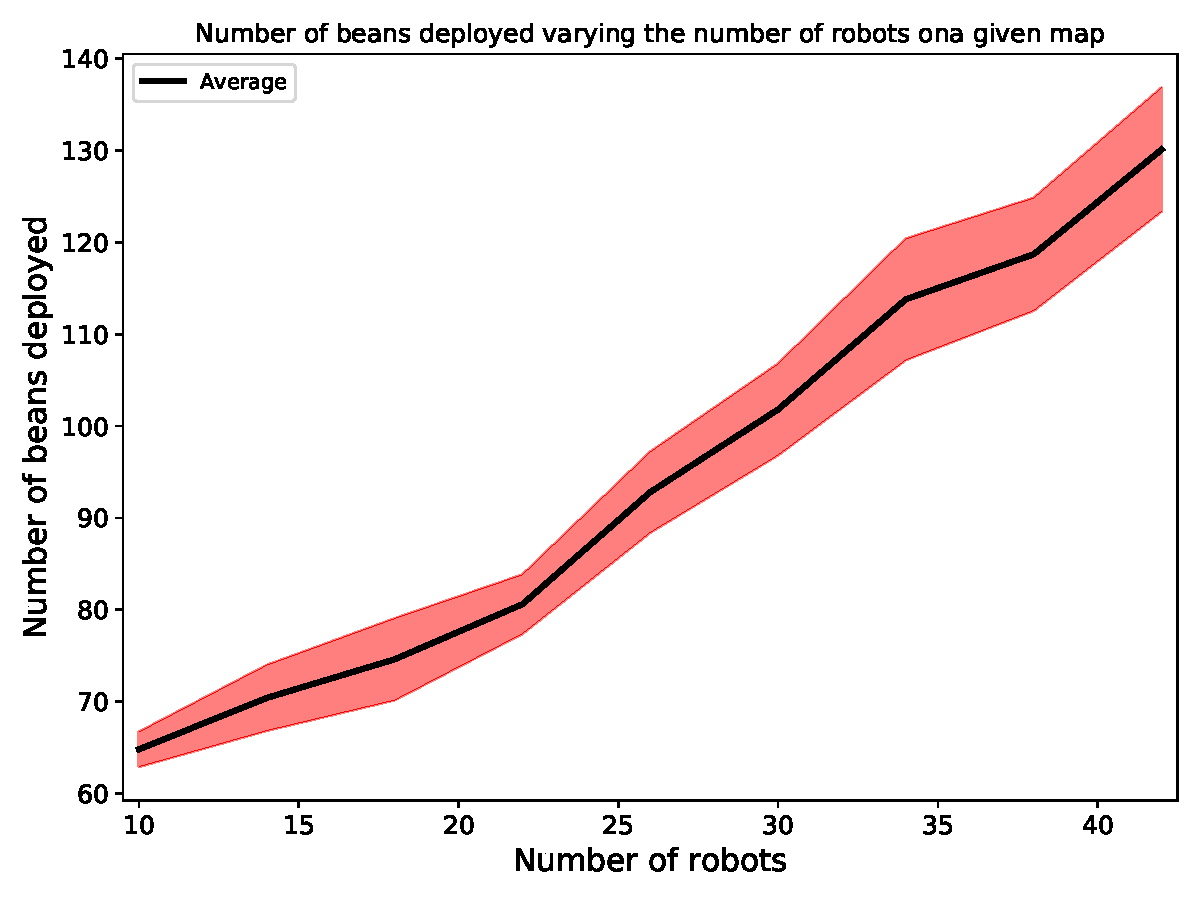
\includegraphics[width=0.9\linewidth]{images/macro_results/robots_beans}
	\caption{In Figura è rappresentato come il numero di robot influisce il numero di ripetitori rilasciati nel territorio. Sull'asse delle \textit{x} è presente il numero di robot e sull'asse delle \textit{y} il numero di ripetitori disposti. Sono state effettuate 10 simulazioni per ogni valore di numero di robot, in nero è presente la media del numero di ripetitori rilasciati e l'area rossa indica la deviazione standard.}
	\label{fig:robotsbeans}
\end{figure}

Invece, rispetto alla seconda analisi effettuata, si evidenzia che il valore di fitness è quello definito nella Formula \ref{math:pso}.
Per quanto riguarda i risultati ottenuti mostrati in Figura \ref{fig:fitness} si nota come con un numero di robot basso la fitness diminuisce velocemente perché il tempo di esplorazione del territorio diminuisce significativamente; al contrario, con un numero elevato di agenti il valore di fitness diminuisce molto più lentamente perché il tempo di esplorazione non subisce diminuzioni significative e nel mentre vi è un numero sempre maggiore di robot in stato di \textit{idling} mentre ci si approccia al termine dell'esplorazione.
Si fa presente, che i valori rappresentati dai segni tondi in rosso sono il valore medio di fitness che si ha ottenuto con tale numero di robot, invece, le barre nere (poco visibili) indicano la variazione data dalla deviazione standard; il fatto che spesso non si vedano è dato da fatto che la deviazione standard è molto bassa.
Considerando il grafico mostrato e concentrandosi sull'intervallo tra i 51 e 76 robot, ci si pone una domanda aperta a cui servirebbero analisi di costi successive e non fattibili nei termini di questo lavoro: “vale la pena utilizzare 10, 15 o addirituttra 25 robot in più se il valore di fitness e il tempo di esplorazione diminuiscono poco significativamente?”.\\
Pensiamo che per rispondere a questa domanda (escludendo i dibattiti etici a riguardo) sia necessario fare delle analisi tenendo conto il costo di realizzazione dei robot e di quanti robot si hanno a disposizione nella pratica e se sia necessario intervenire su un solo quartiere o più quartieri.
\begin{figure}
	\centering
	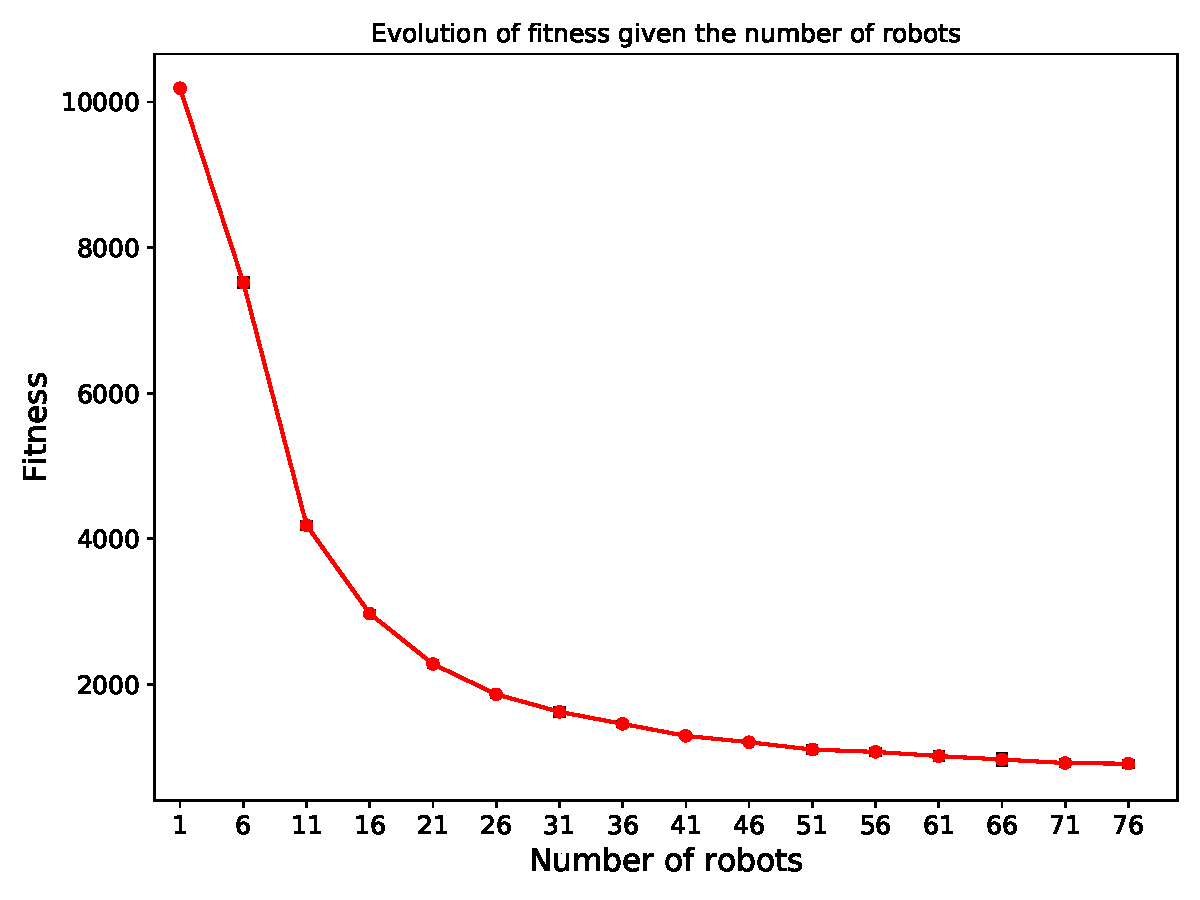
\includegraphics[width=0.9\linewidth]{images/macro_results/fitness}
	\caption{Sull'asse delle \textit{x} è indicato il numero di robot, su quello delle \textit{y} il valore di fitness. Poiché per ogni valore sono state effettuate 10 simulazioni, i valori rappresentati sono la media invece in nero sono le barre di errore date dalla deviazione standard, risultano poco visibili poiché i valori di deviazione standard sono molto piccoli rispetto alle scale del grafico.}
	\label{fig:fitness}
\end{figure}

\subsection{Dimensioni della mappa \textit{vs} numero di ripetitori rilasciati}
\todo[inline]{Non ho trovato il csv che ha generato tale immaigne, quindi controlla tutto quello che ho detto, soprattutto che abbiamo fatto 10 simulazioni per ogni dimensioni. Devi esserne certo, non andare a memroia DP}
Per la produzione di questa analisi, sono state effettuate 10 simulazioni per ogni dimensione della mappa considerata, le mappe sono state generate casualmente ad ogni simulazione, i parametri sono stati utilizzati quelli inferiti dal processo di ottimizzazione (si veda il Capitolo \ref{chap:pso}), il raggio dei ripetitori pari a 3 celle e i feriti erano in grado di poter segnalare la loro presenza. \todo{il numero di robot quant'era? DP}.
I risultati mostrati in Figura \ref{fig:beans}, dove la linea nera è la media e l'area in rosso rappresenta la deviazione standard, mostrano che all'aumentare della dimensione del territorio il numero di ripetitori aumenta (come ragionevole) in maniera assimilabile qualitativamente ad una crescita quadratica.
Questo risultato è più che ragionevole considerando che l'aumentare della dimensione del lato dalla mappa fa aumentare la dimensione di un quadrato portando quindi ad una crescita quadratica delle dimensioni che si riflette coerentemente nel numero di ripetitori necessari.
È interessante notare, aggregando questo dato a quello presentato nella Sotto-sezione \ref{subsec:nrobots}, che l'aumento del numero di ripetitori disposti viene influenzato maggiormente dal numero di agenti impiegati e dal fatto che non si coordinano tra loro rispetto alle dimensioni effettive della mappa che implica una crescita che è intrinseca con l'aumento delle dimensioni della mappa.
\begin{figure}
	\centering
	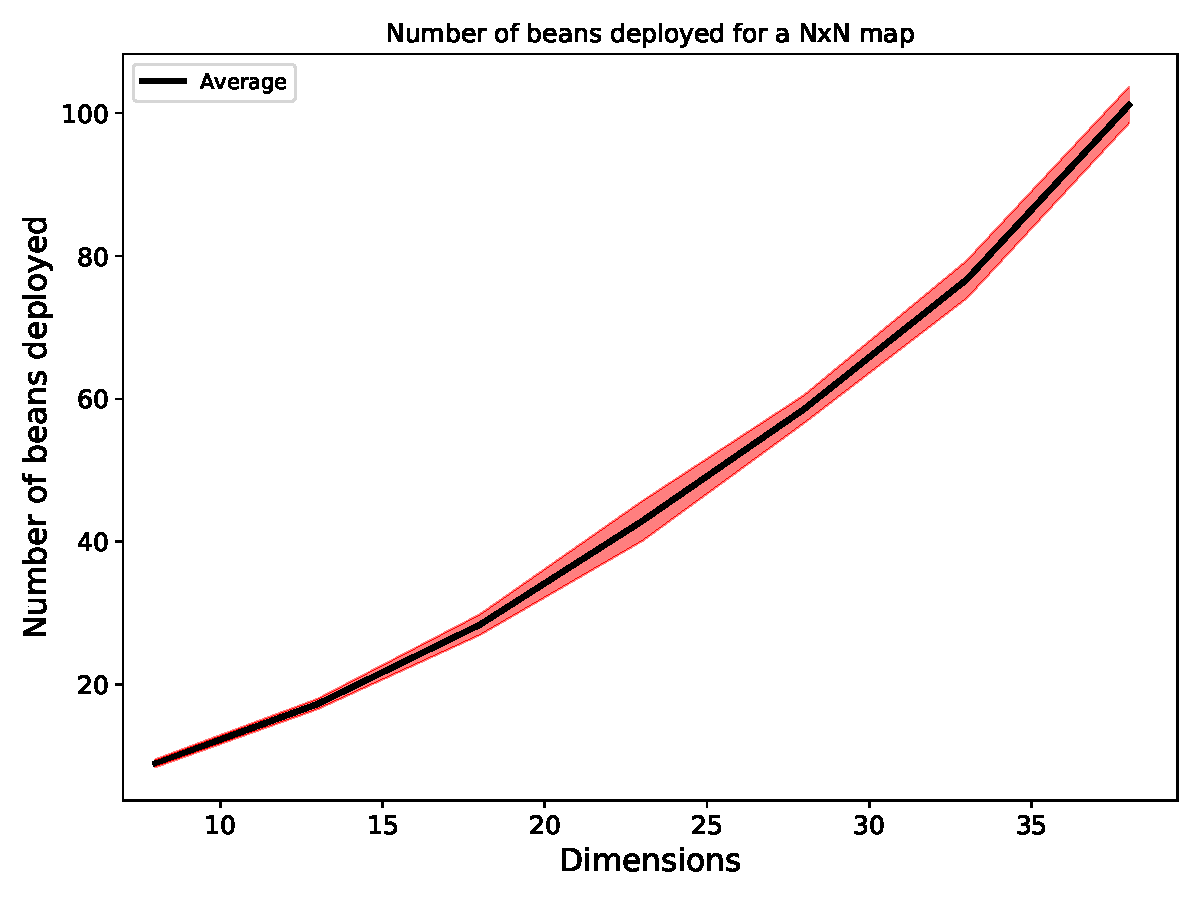
\includegraphics[width=0.9\linewidth]{images/macro_results/beans}
	\caption{Figura che rappresenta come all'aumentare delle dimensioni del territorio (sull'asse delle \textit{x} è rappresentata la dimensione del lato della mappa) aumenta il numero di ripetitori (sull'asse delle \textit{y}) necessari per coprire tutta l'area. In nero è rappresentato il valore medio, mentre in rosso la deviazione standard.}
	\label{fig:beans}
\end{figure}

\subsection{Difficoltà della mappa \textit{vs} tempo richiesto}
\todo[inline]{Mi confermi che i dati sono quelli nel csv robot\_step\_difficulty.csv? DP}
Per tale studio, sono state effettuate un totale di 7 simulazioni in cui si è fatto aumentare la dimensione della mappa, e con esso in maniera proporzionale il numero di robot impiegati, in modo tale da far aumentare la difficoltà complessiva; per difficoltà complessiva si intende la somma delle difficoltà di ogni singola cella.
Le mappe sono state generate casualmente e si è deciso di non effettuare più simulazioni per ogni difficoltà per non complicare inutilmente il grafico e il processo di generazione dati in aggiunta a tutto il tempo richiesto da tali simulazioni; inoltre, i risultati ottenuti da queste poche simulazioni sono stati considerati soddisfacenti per delle analisi di massima.\todo{sicuramente da sistemare. DP}
Siamo anche convinti che effettuare analisi di fino su queste quantità richiederebbero di prendere in considerazione un numero evelato di fattori e i risultati prodotti potrebbero non risultare altamente interessanti, soprattutto contando che nella pratica ogni situazione sarà unica e poco prevedibile a priori.\\
Per quanto riguarda i risultati riportati in Figura \ref{fig:difficulty} , si nota che anche in questo caso l'aumento di \textit{step} richiesti per completare l'esplorazione non è lineare rispetto alla difficoltà ma presenta piuttosto un andamento più assimilabile a quello di un logaritmo.
In aggiunta a tale prima analisi non è possibile trarre altre conclusioni significative, servirebbero molte più simulazioni e sarebbe necessario definire una strategia complicata per poter tenere in considerazioni più fattori per proporre un'analisi approfondita di tale relazione.
\begin{figure}
	\centering
	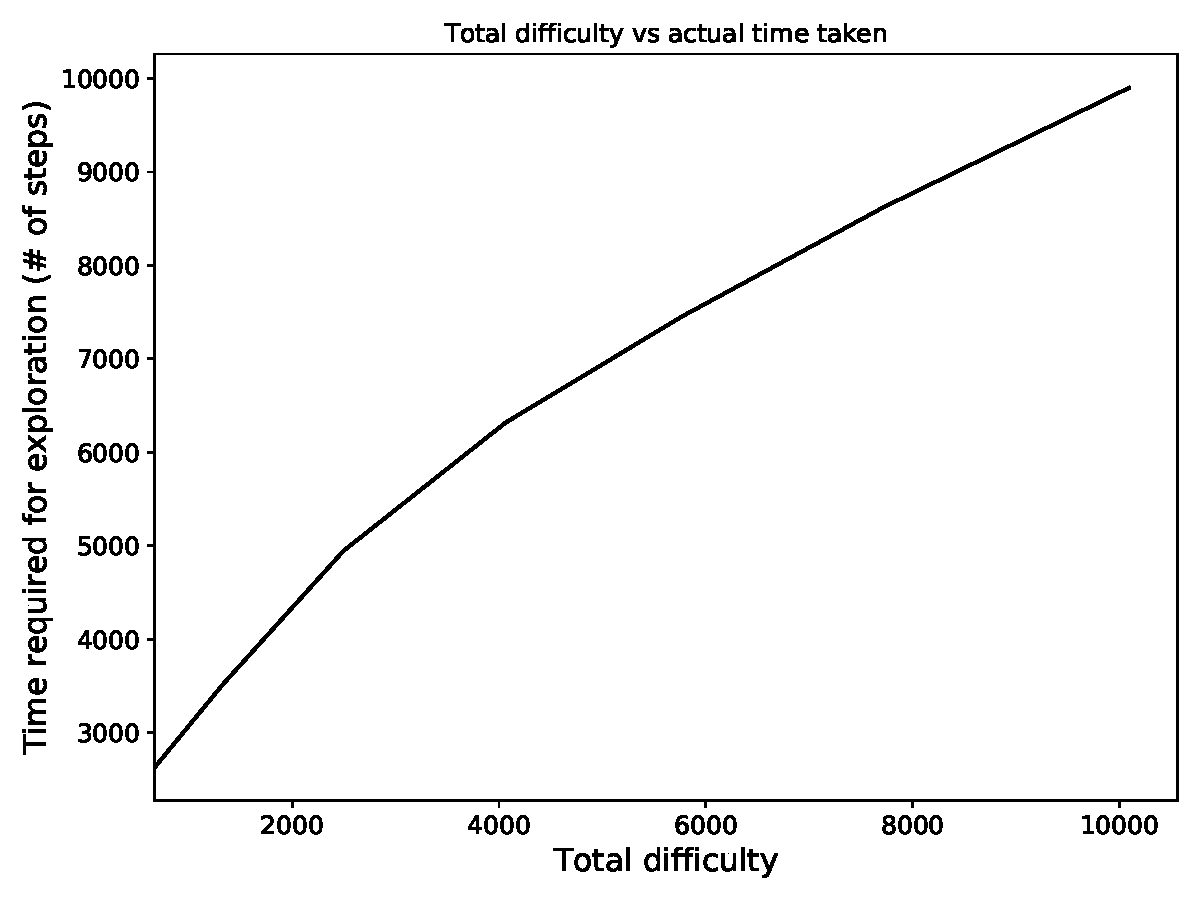
\includegraphics[width=0.9\linewidth]{images/macro_results/difficulty}
	\caption{Sull'asse delle \textit{x} è presente la difficoltà complessiva di esplorazione della mappa e sull'asse delle \textit{y} il numero di \textit{step} effettuati per completare l'esplorazione.}
	\label{fig:difficulty}
\end{figure}

\section{Analisi del parametro $\alpha$}
\label{sec:alpha}
Nelle seguenti analisi si è voluto studiare come al variare del parametro $\alpha$ variasse la scelta delle celle obiettivo da parte dei robot (si ricorda la strategia di scelta della cella descritto nella Sotto-sezione \ref{sub:robots} e della Formula \ref{math:info-gain}), ovvero come il peso introdotto da $\alpha$ fa variare l'importanza che gli agenti danno alla scelta dei cammini.
Come già detto, ci si aspetta che per valori di $\alpha$ elevati si scelgano celle il cui cammino per raggiungerle abbia un costo basso, e per valori di $\alpha$ bassi i robot scelgano principalmente in base all'utilità (e priorità) della cella.\\

In questa parte di lavoro, sono state effettuate due tipi di analisi: in primo luogo, si sono studiati i costi dei cammini scelti durante tutta la durata della simulazione aggregando i risultati di varie simulazioni con lo stesso valore di $\alpha$; in seguito, si è scesi più nel dettaglio andando a valutare come i costi variano all'evolvere del tempo (in termini di \textit{step}) per ogni valore di $\alpha$ studiato in precedenza.
Tutte le simulazioni effettuate per queste analisi sono state eseguite nel seguente modo:
\begin{itemize}
	\item la dimensione della mappa è 30$\times$30 celle con 6 robot disposti all'esplorazione;
	\item il valore di $\gamma$ pari a 0.65 (inferito dal processo di ottimizzazione);
	\item il raggio di percezione pari a 6 celle (anche questo inferito dal processo di ottimizzazione);
	\item il raggio dei ripetitori \textit{wi-fi} pari a 3 celle, in modo da tenerlo proporzionale con la riduzione in scala della mappa rispetto alle dimensioni iniziali che si erano pensate.
\end{itemize}
Infine, per ogni valore di $\alpha$ sono state effettuate 10 simulazioni su mappe scelte casualmente da un insieme di 5 mappe pregenerate in modo \textit{randomico}, le quali non presentano casi patologici.

I risultati delle analisi aggregate sono mostrate in Figura \ref{fig:alphaVar}, in particolare nella Figura \ref{sfig:alphaVarAll} viene mostrata la media dei valori medi (in nero) e relative medie delle deviazioni standard (in rosso) dei costi dei cammini scelti al variare di $\alpha$, la linea tratteggiata rappresenta il valore massimo di deviazione standard dei costi che si è rilevato durante una simulazione.
Poiché i valori di $\alpha$ sono stati studiati con ordini di grandezza differenti (da $10^{-4}$ a $10$), è stato necessario produrre un altro grafico che si concentrasse solo sui valori di $\alpha$ molto piccoli; tale grafico viene mostrato in Figura \ref{sfig:alphaVar0.005}, dove la rappresentazione grafica segue la semantica utilizzata per il grafico precedente.
Dai grafici si nota che per valori relativamente alti di $\alpha$ il costo medio rimane pressoché costante, questo perché nel momento in cui $\alpha$ è sufficiente a far pesare, anche solo in piccola parte, il costo del cammino nel calcolo dell'\textit{info-gain}, le celle in prossimità dell'agente saranno quelle che tipicamente possiedono un valore di \textit{info-gain} maggiore e verranno quindi preferite dall'agente, portando così a costi di spostamento ridotti.
Al contempo, si può apprezzare come all'aumentare del parametro, nonsotante la media rimanga invariata, la deviazione standard e relativo massimo diminuscano, evidenziando che i robot tenderanno sempre più a preferire le celle più economiche da raggiungere a discapito di una loro utilità e priorità bassa.
Si può dedurre che valori di $\alpha$ troppo elevati rendano inutili le politiche di prioritizzazione delle celle e le strategie di gestione delle utilità, poiché gli agenti preferiranno sempre e solo la cella più economica da raggiungere, ignorando gli altri due parametri.
Infine, in Figura \ref{sfig:alphaVar0.005} si può notare come per un valore di $\alpha$ pari a zero il costo venga completamente ignorato (come ci si aspetta) e quindi le celle scelte dipendono unicamente dalla loro utilità e priorità, causando quindi lo spostamento degli agenti per il territorio, cercando semplicemente la cella con utilità e priorità maggiore. Questo porta ad un drastico aumento del numero di \textit{step} necessari a completare la simulazione, in quanto la maggior parte del tempo è impiegato per lo spostamento dei robot.
\begin{figure}
	\subfloat[Media dei costi dei cammini scelti da parte degli agenti durante un insieme di simulazioni con un determinato valore di $\alpha$, relative deviazioni standard e massima deviazione standard presente in una simulazione. In questa figura sono rappresentati i dati relativi a tutti i valori del parametro analizzati.\label{sfig:alphaVarAll}]{
		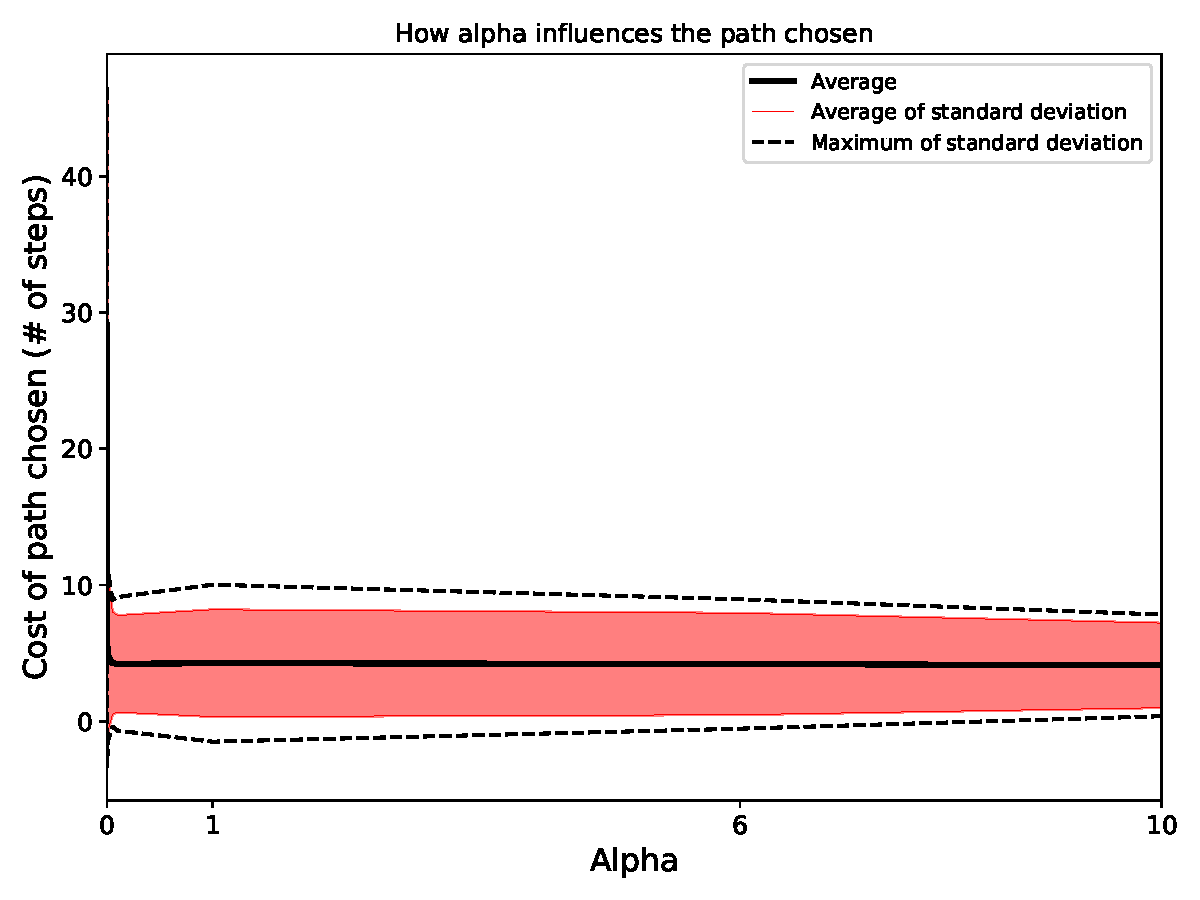
\includegraphics[width=.47\linewidth]{images/alpha_results/variation_all}
	}
	\hfill
	\subfloat[Media dei costi dei cammini scelti da parte degli agenti durante un insieme di simulazioni con un determinato valore di $\alpha$, relative deviazioni standard e massima deviazione standard presente in una simulazione. In questa figura sono rappresentati i dati relativi ai valori del parametro pari a 0, $10^{-4}$, $5\times10^{-4}$, $10^{-3}$, $5\times10^{-3}$.\label{sfig:alphaVar0.005}]{
		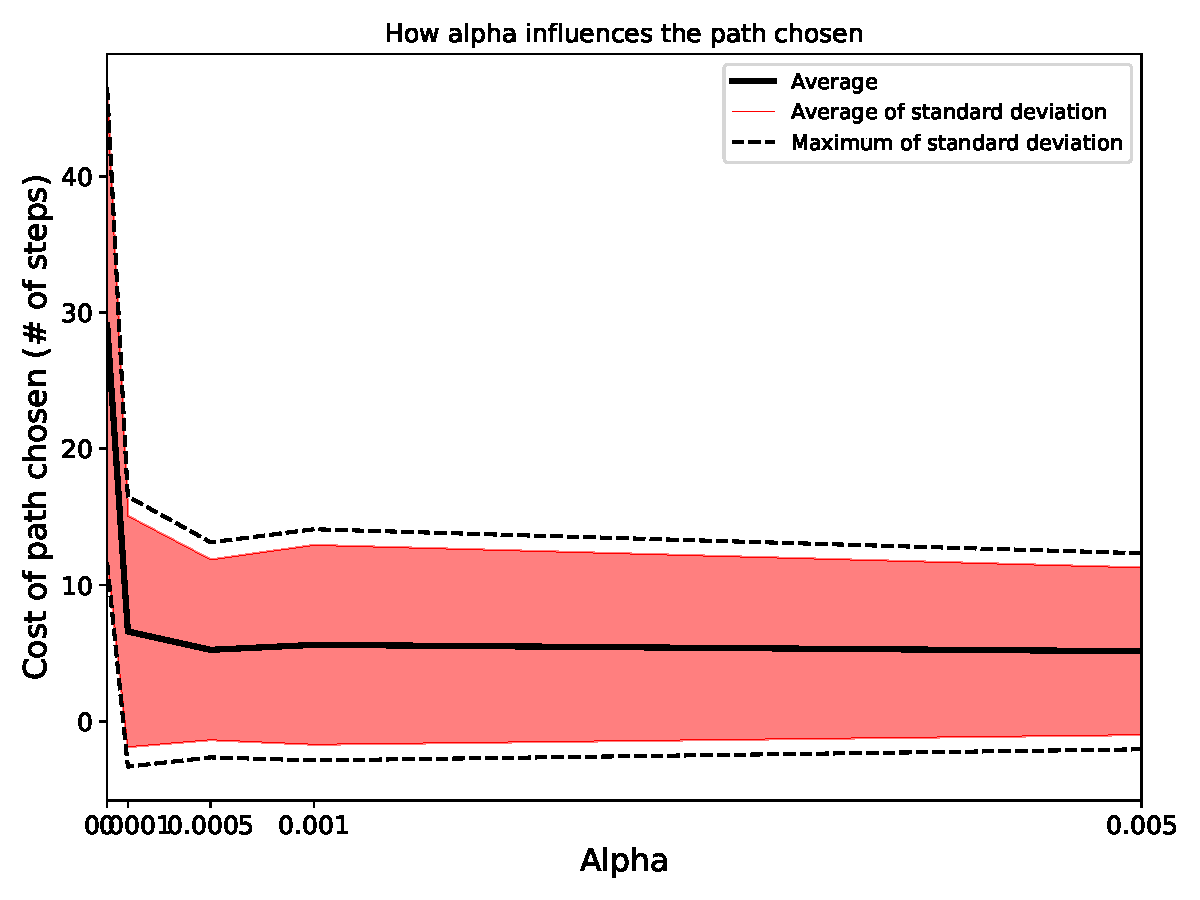
\includegraphics[width=.47\linewidth]{images/alpha_results/variation_0_005}
	}
	\caption{Per entrambi i grafici, in nero è rappresentata la media delle medie dei costi durante le singole simulazioni effettuate con un determinato valore di $\alpha$, in rosso si rappresenta la media delle deviazioni standard calcolate per ogni simulazione ed infine la riga tratteggiata indica il massimo delle deviazioni standard delle simulazioni per il relativo valore di $\alpha$.}
	\label{fig:alphaVar}
\end{figure}

Poiché le analisi precedentemente introdotte aggregano i dati in modo sostanziale, si è deciso di analizzare più nello specifico come $\alpha$ influisse nella scelta dei cammini durante la simulazione, in particolare per ogni valore di $\alpha$ preso in considerazione nella parte precedente si è valutato per ogni \textit{step} della simulazione i costi dei cammini scelti dagli agenti.
Si sono considerati solo gli \textit{step} in cui almeno un robot ha effettuato la scelta della cella \textit{target} e se più robot hanno effettuato una scelta nello stesso \textit{step}, si è considerata la media di essi; tale studio è stato effettuato aggregando le varie simulazioni per lo stesso valore del parametro. 
Con il termine aggregazione intendiamo in questo caso andare a valutare contemporaneamente per ogni \textit{step} cosa è successo durante le varie simulazioni.
I grafici per alcuni valori di $\alpha$ che sono stati ritenuti significativi sono stati riportati in Figura \ref{fig:alphaOverTime}, invece, mentre per i grafici dei restanti valori si rimanda all'Appendice \ref{apx:alpha}. Si noti che, per rendere i grafici leggibili, sono stati accorpati i valori dei costi per intervalli di 100 \textit{step} l'uno; di conseguenza viene rappresentata la media (evidenziata dalla curva colorata) e in nero gli \textit{errorbar} dati dalle relative deviazioni standard.
Dai grafici si nota come per un valore di $\alpha$ pari a zero (Figura \ref{sfig:alphaCost0}) il costo medio dei cammini rimane elevato durante l'intera simulazione e vi è un'alta varianza attorno a tale valore. Come già affermato in precedenza, in questa situazione gli agenti scelgono la cella in base alla sua utilità e priorità, ignorando completamente i costi; di conseguenza i robot tenderanno a muoversi per lunghe distanze attraverso il territorio, portando uno stesso robot a dover ripercorre tratti di strada più volte.
Tale affermazione viene ampiamente sostenuta dall'evoluzione che mostra il grafico preso in considerazione, dove il costo varia ampiamente e, come vedremo in seguito, l'esplorazione dell'area richiede molto più tempo del solito.
Per quanto riguarda, invece, un valore di $\alpha$ pari a $10^{-2}$ (si faccia riferimento alla Figura \ref{sfig:alphaCost0.01}), si può notare come i tempi di esplorazione diminuiscono significativamente e anche i costi risultano in media molto più bassi; tale risultato accredita ulteriormente l'affermazione precedente.
In aggiunta si sottolinea che per valori poco più alti, i costi dei cammini minimi diminuiscono in maniera ancora più drastica (si veda in Appendice la Figura \ref{sfig:alpha0.05}).
Per quanto concerne valori di $\alpha$ pari a 6 e 10 (rispettivamente in Figura \ref{sfig:alphaCost6} e \ref{sfig:alphaCost10}) si nota come il costo medio diminuisce ulteriormente, salvo aumentare (come già succedeva per valori pari a $10^{-2}$ e superiori) durante le ultime fasi dell'esplorazione, dove si suppone che siano rimaste solo le celle con utilità molto bassa o accerchiate da celle di difficile attraversamento che hanno scoraggiato la loro scelta da parte degli agenti finché avevano a disposizione un'alternativa. I robot vanno quindi ad esplorare quelle celle che erano state evitate durante un primo passaggio a causa dell'elevato costo o della bassa utilità.
Al contempo, si può notare come la deviazione standard per un valore del parametro pari a 6 sia minore rispetto ad un valore pari a 10; possiamo supporre che questo sia il motivo principale per cui il processo di ottimizzazione abbia optato per un valore di $\alpha$ intermedio tra i due.\\
Per concludere, sono stati messi a confronto i costi medi dei percorsi scelti durante ogni simulazione, confrontando complessivamente i dati analizzati separatamente in precedenza.
I risultati sono proposti in Figura \ref{fig:alphaComparison}, dove si nota come per un valore del parametro pari a 0 i costi sono estremamente più alti e questo implica tempi di completamente dell'esplorazione maggiori. In aggiunta, per valori di $\alpha$ molto bassi, la media dei costi iniziali è significativamente più alta rispetto agli altri valori.
Infine, si nota come per valori di $\alpha$ pari ad uno e sei i tempi di esplorazione siano leggermente inferiori rispetto a quelli richiesti dagli altri valori.

\begin{figure}
	\begin{tabular}{cc}
		\subfloat[Effetto di un valore del parametro $\alpha$ pari a 0 nella scelta della cella obiettivo in base al costo del cammino.\label{sfig:alphaCost0}]{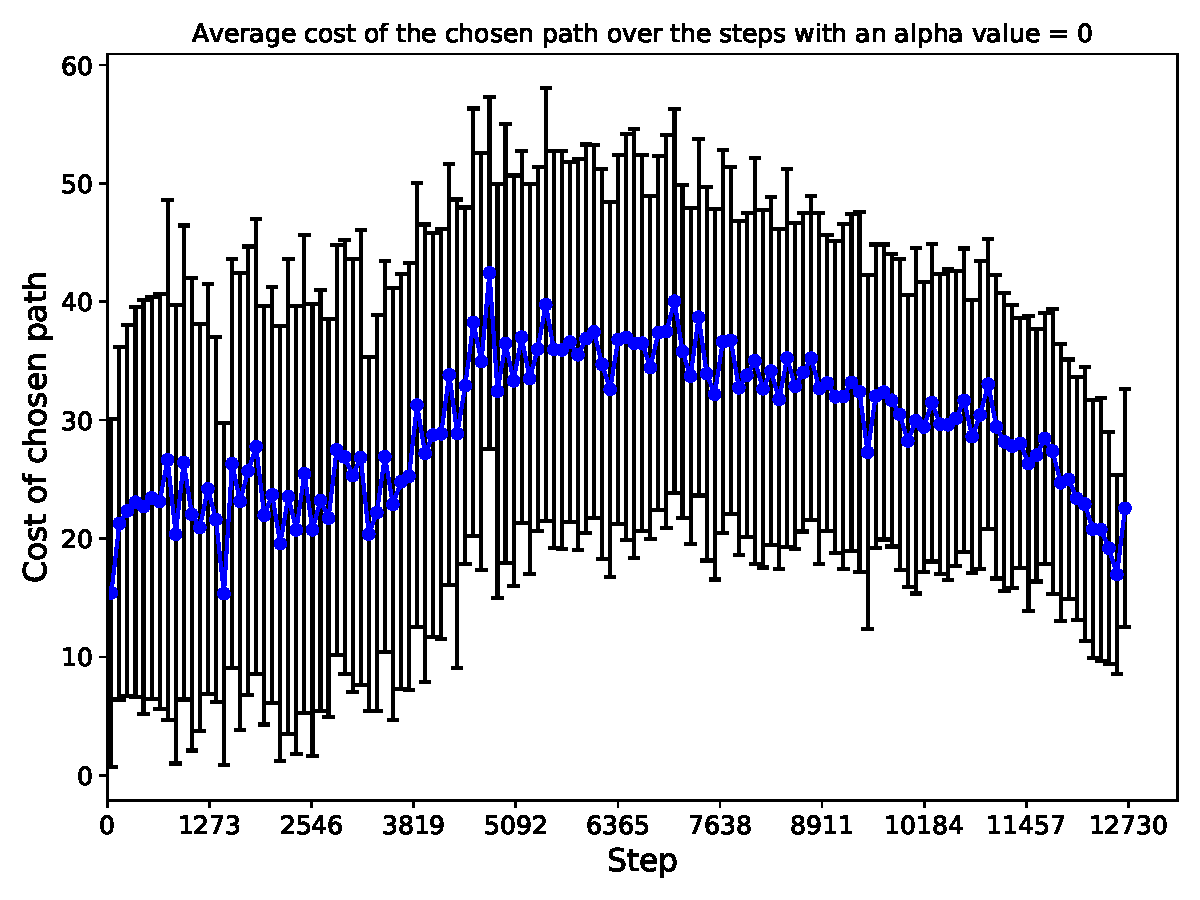
\includegraphics[width = .5\textwidth]{images/alpha_results/cost_alpha_0}} &
		\subfloat[Effetto di un valore del parametro $\alpha$ pari a 0.01 nella scelta della cella obiettivo in base al costo del cammino.\label{sfig:alphaCost0.01}]{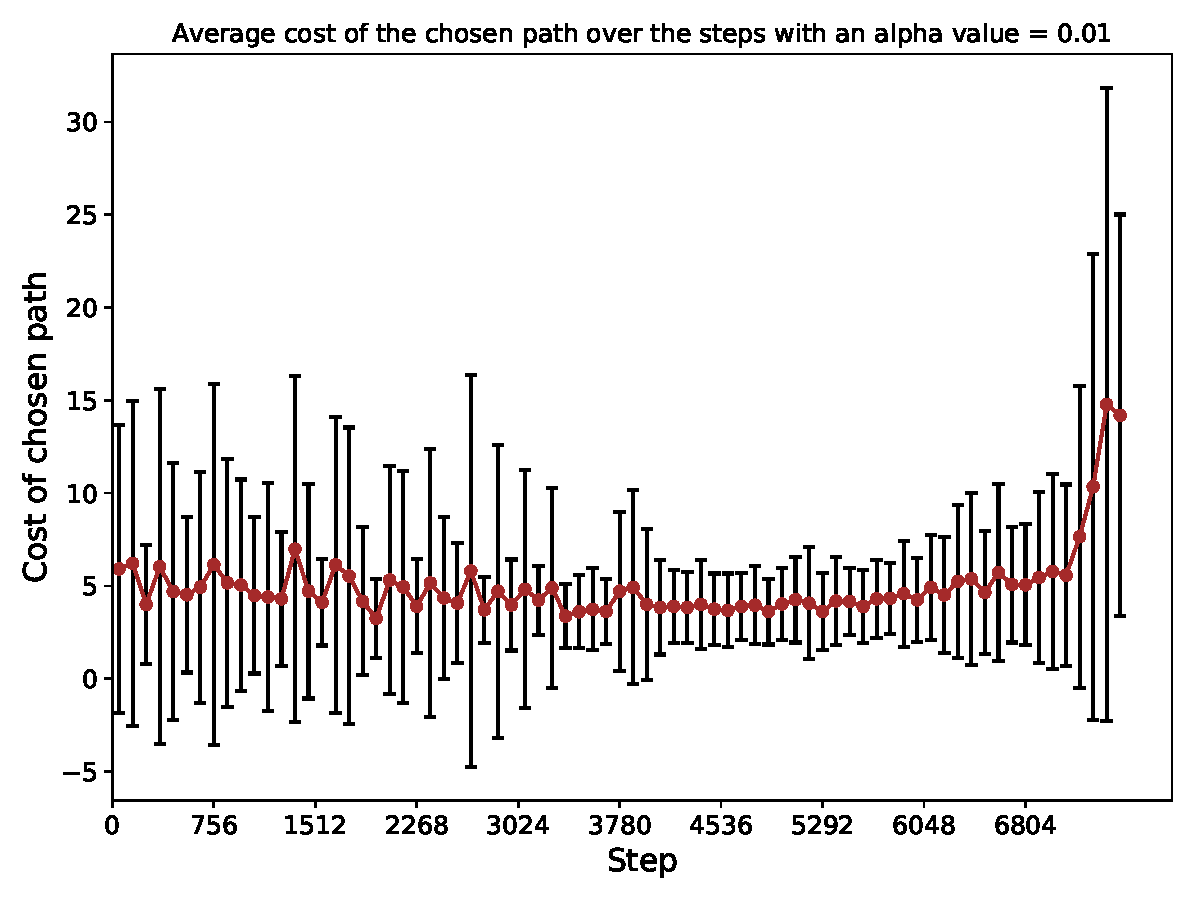
\includegraphics[width = .5\textwidth]{images/alpha_results/cost_alpha_0_01}}\\
		\subfloat[Effetto di un valore del parametro $\alpha$ pari a 6 nella scelta della cella obiettivo in base al costo del cammino.\label{sfig:alphaCost6}]{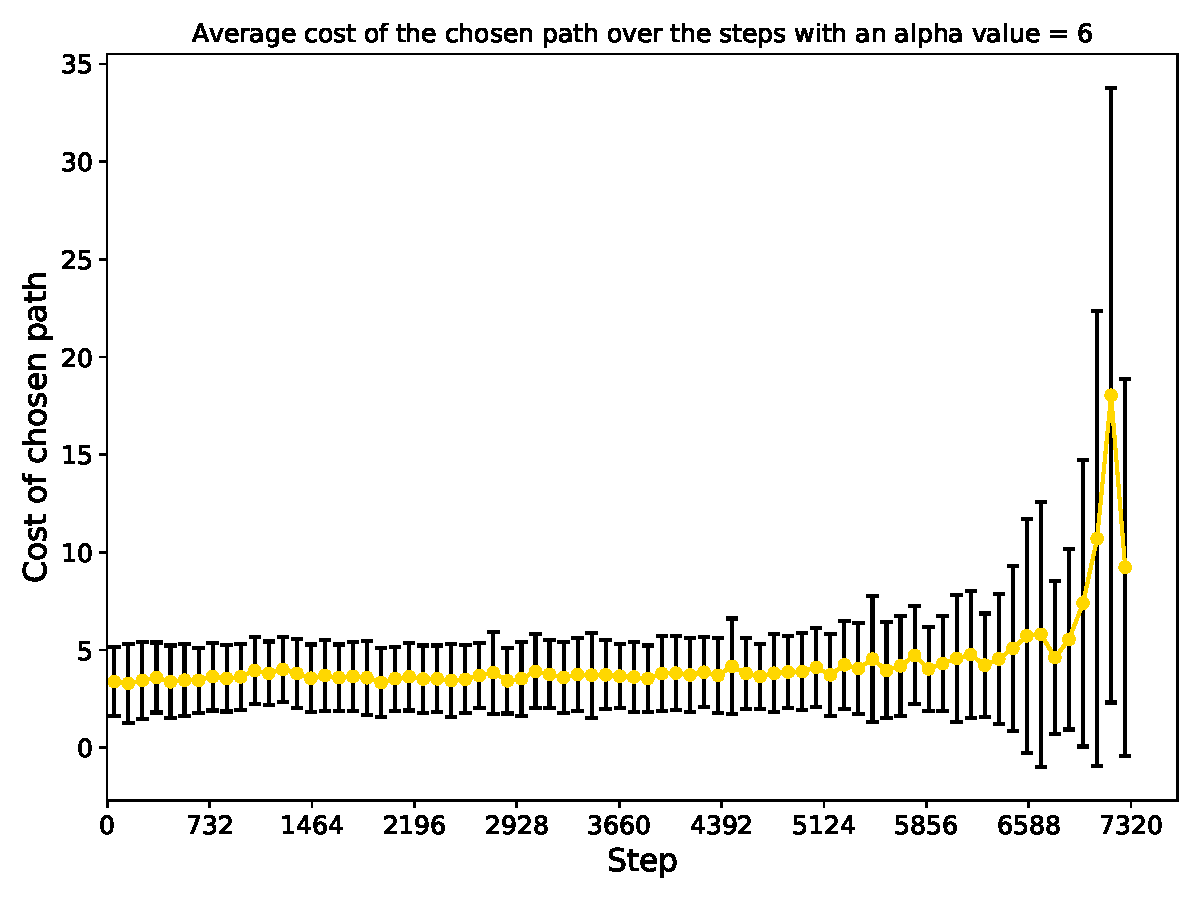
\includegraphics[width = .5\textwidth]{images/alpha_results/cost_alpha_6}} &
		\subfloat[Effetto di un valore del parametro $\alpha$ pari a 10 nella scelta della cella obiettivo in base al costo del cammino.\label{sfig:alphaCost10}]{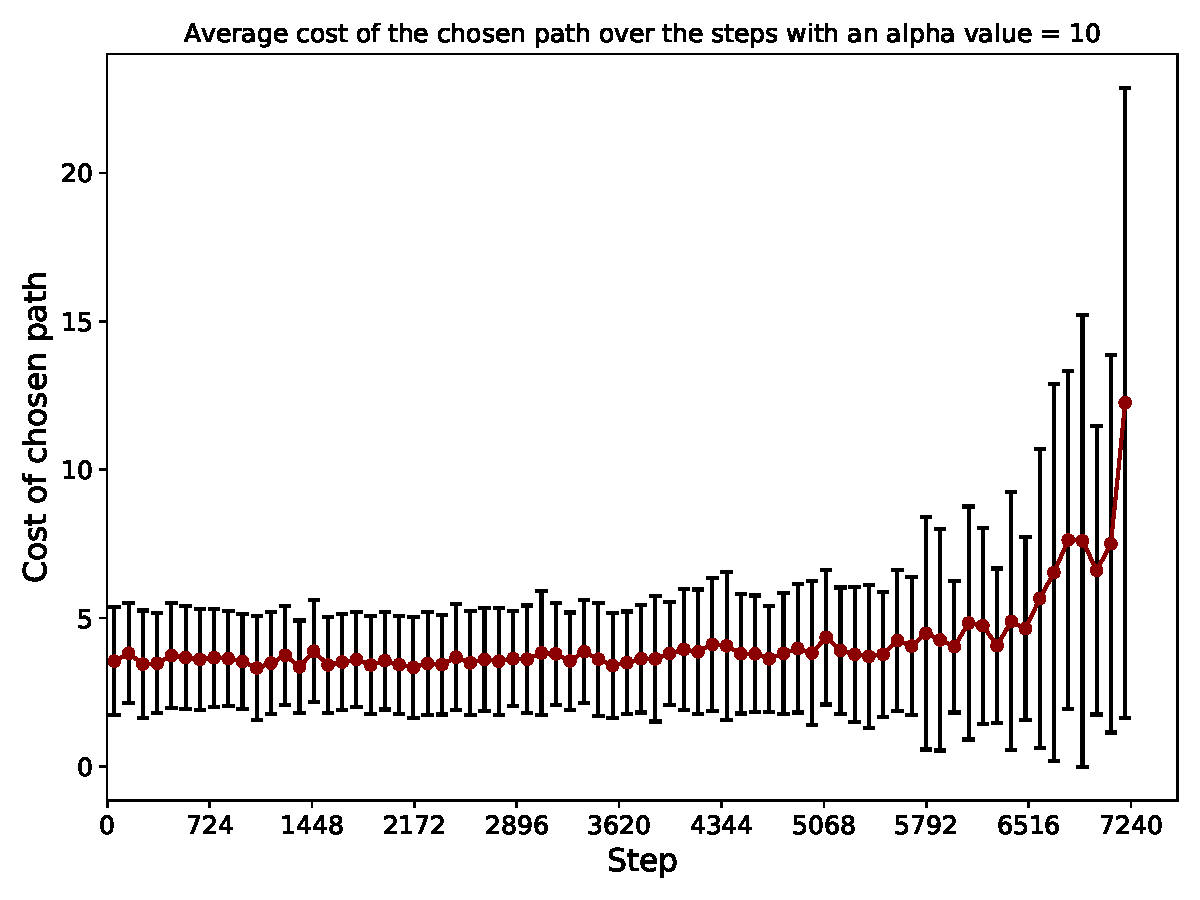
\includegraphics[width = .5\textwidth]{images/alpha_results/cost_alpha_10}}
	\end{tabular}
	\caption{In colore si denota la media dei costi dei cammini per raggiungere la cella scelta, i valori sono stati calcolati aggregando le scelte effettuate durante intervalli di 100 \textit{step}; in nero gli \textit{errorbar} relativi alla media determinati dalla deviazione standard.}
	\label{fig:alphaOverTime}
\end{figure}

\begin{figure}
	\centering
	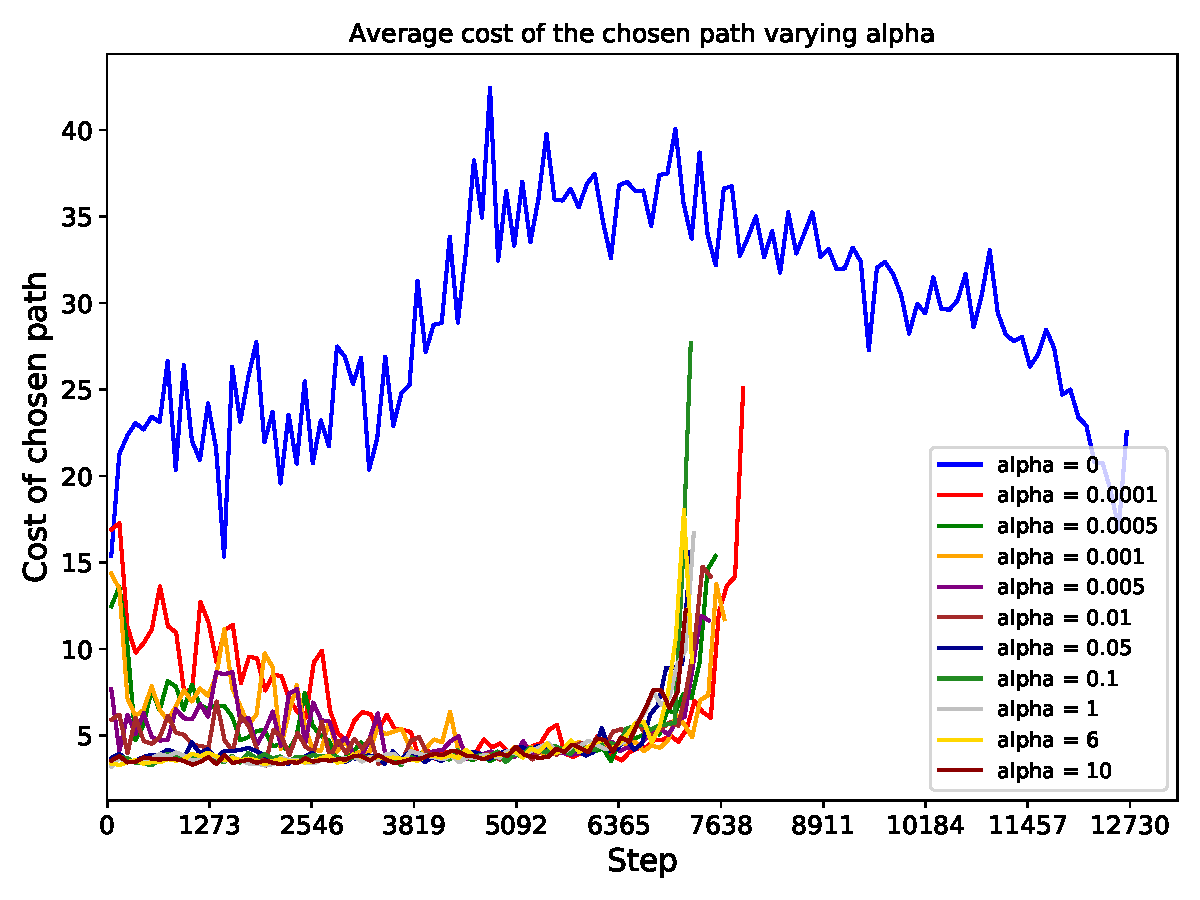
\includegraphics[width=0.9\linewidth]{images/alpha_results/comparison}
	\caption{Confronto tra la media dei costi dei cammini durante la simulazione per diversi valori di $\alpha$, anche in questo caso la media è stata calcolata in intervalli di 100 \textit{step}.}
	\label{fig:alphaComparison}
\end{figure}

\section{Analisi del parametro $\gamma$}
\label{sec:gamma}
Le analisi relative al parametro $\gamma$ sono state effettuate in maniera analoga a quelle precedenti: per ogni valore d'interesse di $\gamma$ sono state effettuate 10 simulazioni ognuna delle quali mantenendo invariati tutti gli altri parametri.
In particolare, le dimensioni della mappa sono state mantenute pari a 30$\times$30 celle, sono stati impiegati 6 robot con un raggio di visione pari a 6 celle, come suggerito dal processo di ottimizzazione descritto nel Capitolo \ref{chap:pso}, un raggio del ripetitore pari a 3 celle e abilitando i feriti a poter segnalare le loro posizioni.
Per quanto riguarda le mappe, sono state sfruttate le 5 mappe generate casualmente e utilizzate per le analisi condotte sul parametro $\alpha$ (Sezione \ref{sec:alpha}).
Infine, poiché ci si è accorti che il valore di $\alpha$ sia in grado di influenzare la distanza che mantengono tra loro i robot, si è deciso di effettuare due batterie di test: una prima in cui si è mantenuto un valore di $\alpha$ basso pari a $10^{-4}$ e poi per uno elevato pari a 8.175 (valore consigliato dal processo di ottimizzazione).
Le due batterie di test sono state eseguite in modo separato e autonomamente l'una dall'altra, non modificando altri parametri (escluso $\gamma$).\\
La metrica utilizzata per valutare come il parametro influisce nel comportamento del modello è stata la distanza media tra i robot. Come già detto, ci si aspetta che per valori alti di $\gamma$ gli agenti tendano a tenersi più distanti tra loro e viceversa.
Formalmente, la metrica viene computata nel seguente modo: per ogni robot si è calcolata la media delle distanze euclidee tra l'agente di interesse e tutti gli altri robot; in seguito, si è computata la media (e relativa deviazione standard) delle distanze medie.
Tale metrica è stata misurata ad ogni \textit{step} della simulazione.
Di seguito, mostriamo i principali risultati ottenuti in entrambe le batterie di test, ulteriori dati prodotti, meno significativi, sono riportati in Appendice \ref{apx:gamma}.

\subsection{Analisi con valore di $\alpha$ basso}
\label{subsec:gammaalow}
Una prima analisi effettuata è stata considerare per ogni valore del parametro la distribuzione della distanza media, ovvero in quanti \textit{step} si è presentato un determinato valore di distanza media; tali distribuzioni sono state calcolando aggregando i dati di tutte le simulazioni per ogni valore del parametro.
In Figura \ref{fig:gammaDistr} sono mostrate le distribuzioni per due valori di $\gamma$ (le altre sono riportate in Appendice \ref{apx:gamma}); si noti che la scala sull'asse delle \textit{y} è logaritmica e la distribuzione è rappresentata solo da un \textit{marker} che indica il numero di \textit{step} in cui si è verificate quel valore di distanza. Si tenga inoltre presente che i valori di distanza sono stati raggruppati per numeri interi.
Nelle distribuzioni mostrate, si nota come che per un valore di $\gamma$ pari a 0.32 (Figura \ref{sfig:gammaDistr0.32}), gli agenti tendano a mantenere una distanza nell'“intorno” di 30, con pochi casi di distanze pari o superiori a 50; al contempo, con un valore pari a 0.65 (Figura \ref{sfig:gammaDistr0.65}), si nota come non vi sia un valore di distanza che viene assunto significativamente più frequentemente di altri, ma il grafico presenta una distribuzione più “liscia”.\\
\begin{figure}
	\subfloat[Distribuzione della distanza media mantenuta dai robot con un valore di $\gamma$ pari a 0.32.\label{sfig:gammaDistr0.32}]{
		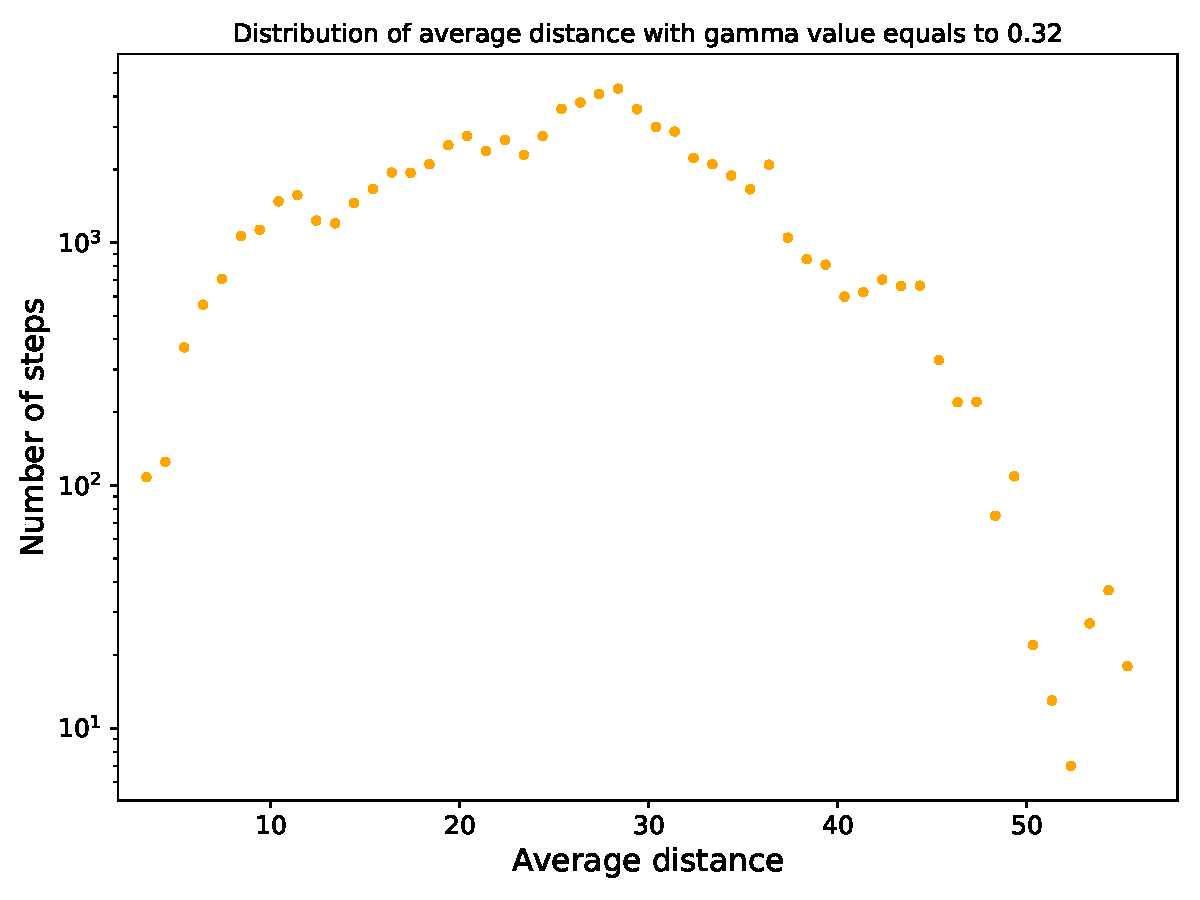
\includegraphics[width=.47\linewidth]{images/gamma_results/low_alpha/distribution_distance_gamma_0_32}
	}
	\hfill
	\subfloat[Distribuzione della distanza media mantenuta dai robot con un valore di $\gamma$ pari a 0.65.\label{sfig:gammaDistr0.65}]{
		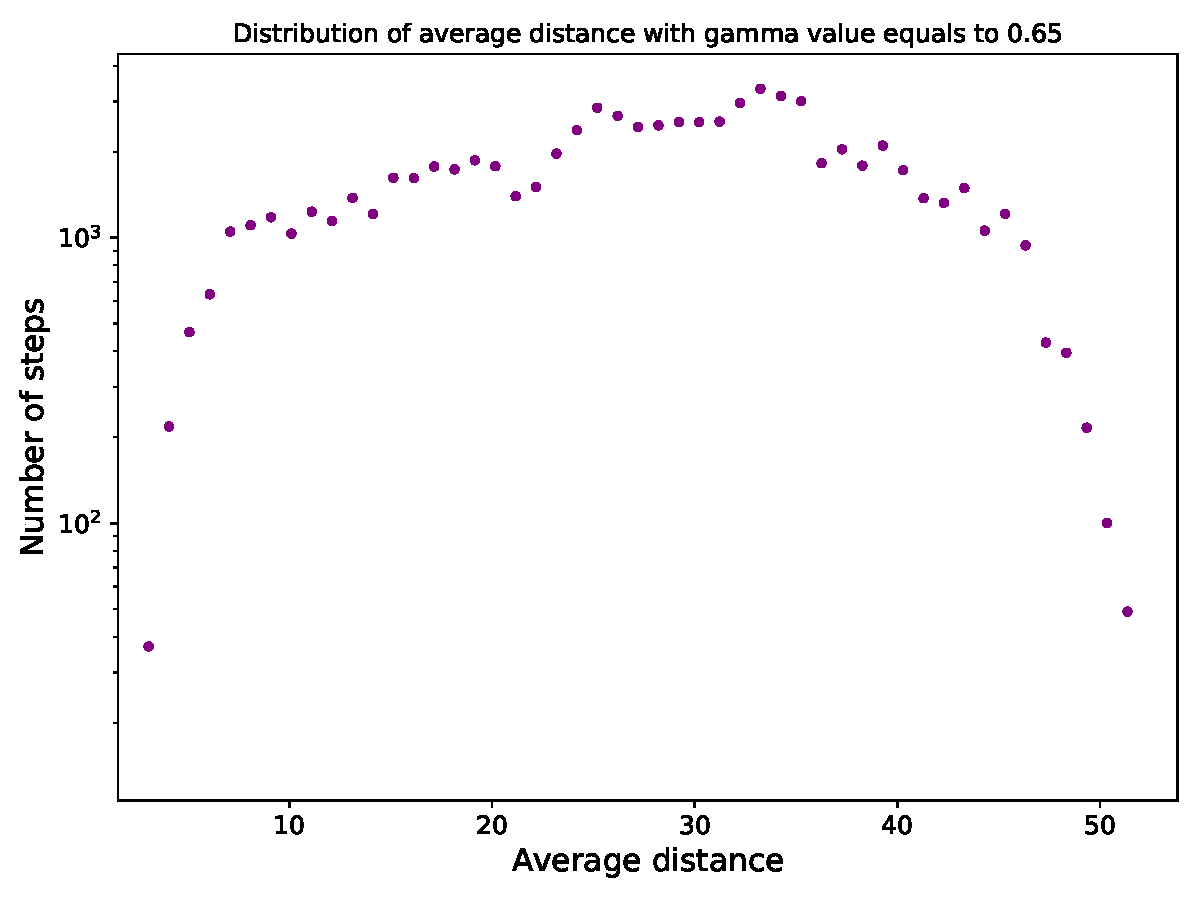
\includegraphics[width=.47\linewidth]{images/gamma_results/low_alpha/distribution_distance_gamma_0_65}
	}
	\caption{Distribuzione della distanza media mantenuta dai robot al variare del valore di $\gamma$, per valutare la distribuzione si è conteggiato in quanti \textit{step} i robot hanno presentato tale distanza, il numero di \textit{bin} per produrre la distribuzione è pari alla differenza tra la distanza minima e massima presente durante la simulazione, tale valore è stato poi arrotondato. Infine si noti che l'asse delle \textit{y} è a scala logaritmica.}
	\label{fig:gammaDistr}
\end{figure}
Poiché effettuare dei confronti solo mediante grafici di distribuzioni realizzati ognuno per ogni valore analizzato di $\gamma$ risulta complicato e poco significativo, si è deciso di confrontarli unendo tali distribuzioni nello stesso grafico; si noti che l'asse delle \textit{y} non è più a scala logaritmica, in modo da favorire un confronto qualitativo delle distribuzioni.
Il grafico complessivo, riportato in Figura \ref{fig:gammaComparison}, mostra come al crescere de valore $\gamma$ la distanza media tra gli agenti tende ad aumentare per un numero maggiore di \textit{step}.
In particolare si può notare come che per valori di $\gamma$ pari a 0.32 e 1 si presentino dei veri e propri “picchi”; è interessante che per il valore pari a 0.65 non vi sia un vero e proprio “picco” ma, come già detto, la distribuzione risulti più “liscia”, presentando al contempo un numero maggiore di \textit{step} con distanze medie tra 40 e 50 (che risultano essere distanze elevate) e che non compaiono in modo così significativo per nessun altro valore di $\gamma$.
Per valori bassi di $\gamma$ non si evidenziano significative differenze in termini di distanza, ma comunque tende ad emergere una concentrazione di valori di distanza relativamente bassi rispetto agli altri valori di $\gamma$.
In particolare, valutando con attenzione la Formula \ref{math:utility-red} grazie a cui l'utilità di una cella viene ridotta, possiamo intuire che un valore basso di $\gamma$ porta tutte le celle percepite dal robot ad avere un'utilità molto simile e prossima allo $0$. Viceversa, un valore alto di $\gamma$ genera una netta differenza tra celle immediatamente circostanti alla posizione e celle più lontane, garantendo un'efficace meccanismo di dissuasione per gli altri robot.\\
Riassumendo quanto valutato fin'ora, si nota come con un valore di $\alpha$ basso, il parametro $\gamma$ influenza la distanza tra gli agenti, presentando un comportamento particolare per il valore di $\gamma$ pari a 0.65 che è stato quello suggerito dal processo di ottimizzazione (si faccia riferimento al Capitolo \ref{chap:pso}).
\begin{figure}
	\centering
	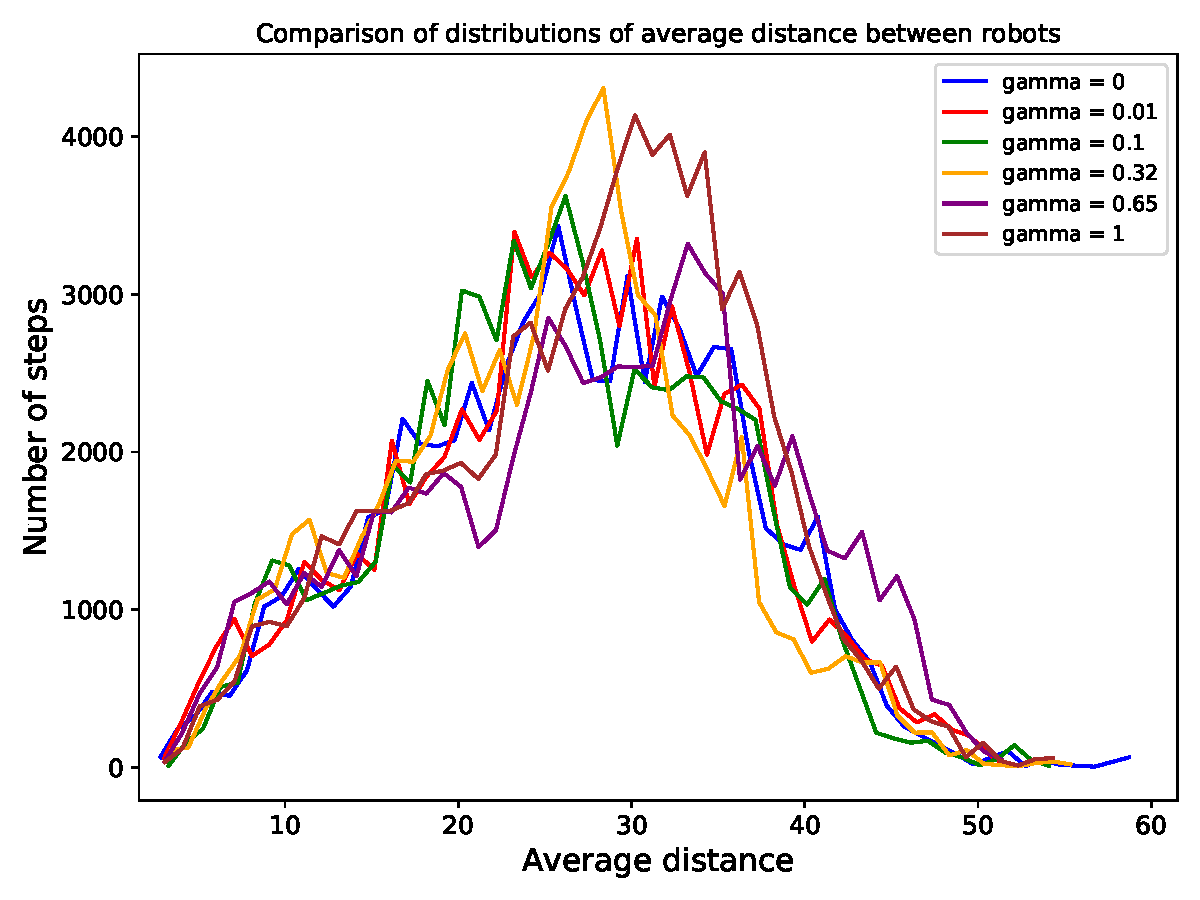
\includegraphics[width=0.9\linewidth]{images/gamma_results/low_alpha/comparison}
	\caption{Grafico che riassume tutte le distribuzioni di distanze medie durante le simulazioni per ogni valore di $\gamma$, si noti che l'asse delle \textit{y} non è più logaritmico.}
	\label{fig:gammaComparison}
\end{figure}

Infine, \margin{Come $\alpha$ influenza la distanza tra gli agenti}si è andati a studiare l'evolversi all'interno della singola simulazione (ne è stata scelta una casualmente tra le dieci eseguite per ogni valore di $\gamma$ studiato) della distanza media tra i robot.
Tali evoluzioni sono mostrate in Figura \ref{fig:gammaSim} per quanto riguarda i valori del parametro pari a 0.32 (Figura \ref{sfig:gammaSim0.32}) e 0.65 (Figura \ref{sfig:gammaSim0.65}), per gli altri si faccia riferimento all'Appendice \ref{apx:gamma}.
In entrambe le simulazioni emerge come più di una volta la distanza tra gli agenti sia diminuita drasticamente e repentinamente per poi, dopo pochi \textit{step}, ricominciare ad aumentare.
Si è associato tale fenomeno alla possibilità da parte dei feriti di segnalarsi, in particolare, ogni volta che qualcuno si segnala, la priorità delle celle del vicinato viene incrementata, e quindi incrementa l'\textit{info-gain} di tali celle.
Notiamo però che questo fenomeno sembra essere meno presente mano a mano che gamma cresce: questo è probabilmente dovuto al fatto che, al crescere di gamma, l'utilità delle celle nell'intorno di una cella che viene esplorata è fortemente diminuito, mentre le celle più distanti subiscono meno questo malus. Nella scelta della cella bersaglio, essendo $\alpha$ molto basso, la differenza tra utilità e priorità di una cella potrebbe propendere verso la prima componente, rendendo quindi una cella proritizzata vicina a una cella già esplorata meno interessante di una priva di priorità ma più distante.
Poiché il valore di $\alpha$ è basso, i robot non faranno pesare in maniera significativa il costo del cammino e quindi, anche se distanti, tenderanno a scegliere tali celle, portando quindi ad un avvicinamento dei robot con lo scopo di esplorare completamente (e in poco tempo) tutta l'area attorno a dove si è segnalato un ferito.
\begin{figure}
	\subfloat[Evoluzione della distanza media tra gli agenti con un valore di $\gamma$ pari a 0.32.\label{sfig:gammaSim0.32}]{
		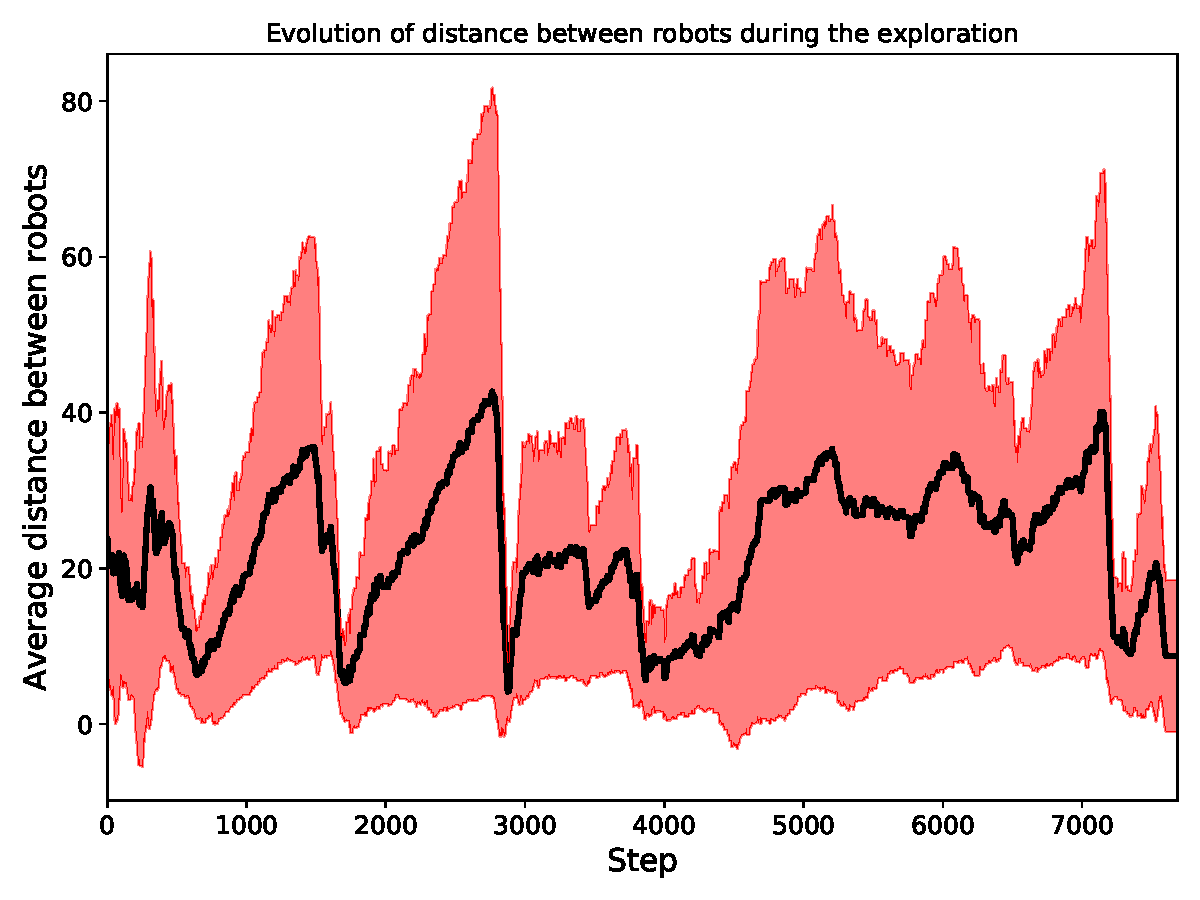
\includegraphics[width=.47\linewidth]{images/gamma_results/low_alpha/dinstance_simulation_gamma_0_32_simid_0}
	}
	\hfill
	\subfloat[Evoluzione della distanza media tra gli agenti con un valore di $\gamma$ pari a 0.65.\label{sfig:gammaSim0.65}]{
		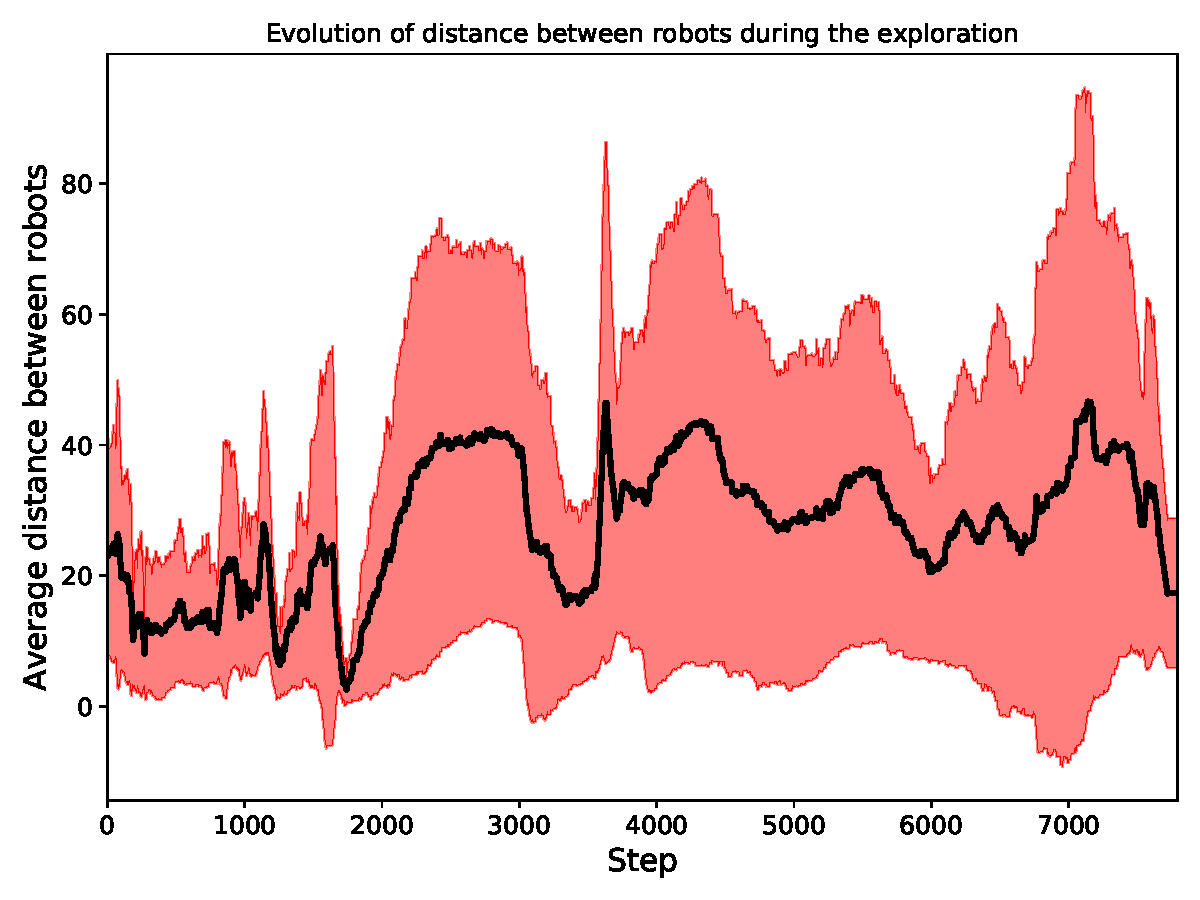
\includegraphics[width=.47\linewidth]{images/gamma_results/low_alpha/dinstance_simulation_gamma_0_65_simid_0}
	}
	\caption{Sull'asse delle \textit{x} si trova il tempo, in termini di \textit{step}, impiegato per l'esplorazione della mappa, mentre sull'asse delle \textit{y} la distanza media tra gli agenti.}
	\label{fig:gammaSim}
\end{figure}

\subsection{Analisi con valore di $\alpha$ alto}
\label{subsec:gammaahigh}
Come in precedenza, le prime analisi effettuate si sono concentrate sulla distribuzione delle distanze medie.
In Figura \ref{fig:gammaHDistr} sono rappresentate le due distribuzioni per i valori di $\gamma$ considerati in precedenza; si può notare che con valori alti di $\alpha$, l'andamento della distribuzione si sia invertita rispetto al caso precedente: per un valore pari a 0.32 (Figura \ref{sfig:gammaHDistr0.32}) la distribuzione sembra essere più “liscia”, invece per un valore pari a 0.65 (Figura \ref{sfig:gammaHDistr0.65}) o superiore sembra infittirsi per alcuni valori di distanza.
\begin{figure}
	\subfloat[Distribuzione della distanza media mantenuta dai robot con un valore di $\gamma$ pari a 0.32.\label{sfig:gammaHDistr0.32}]{
		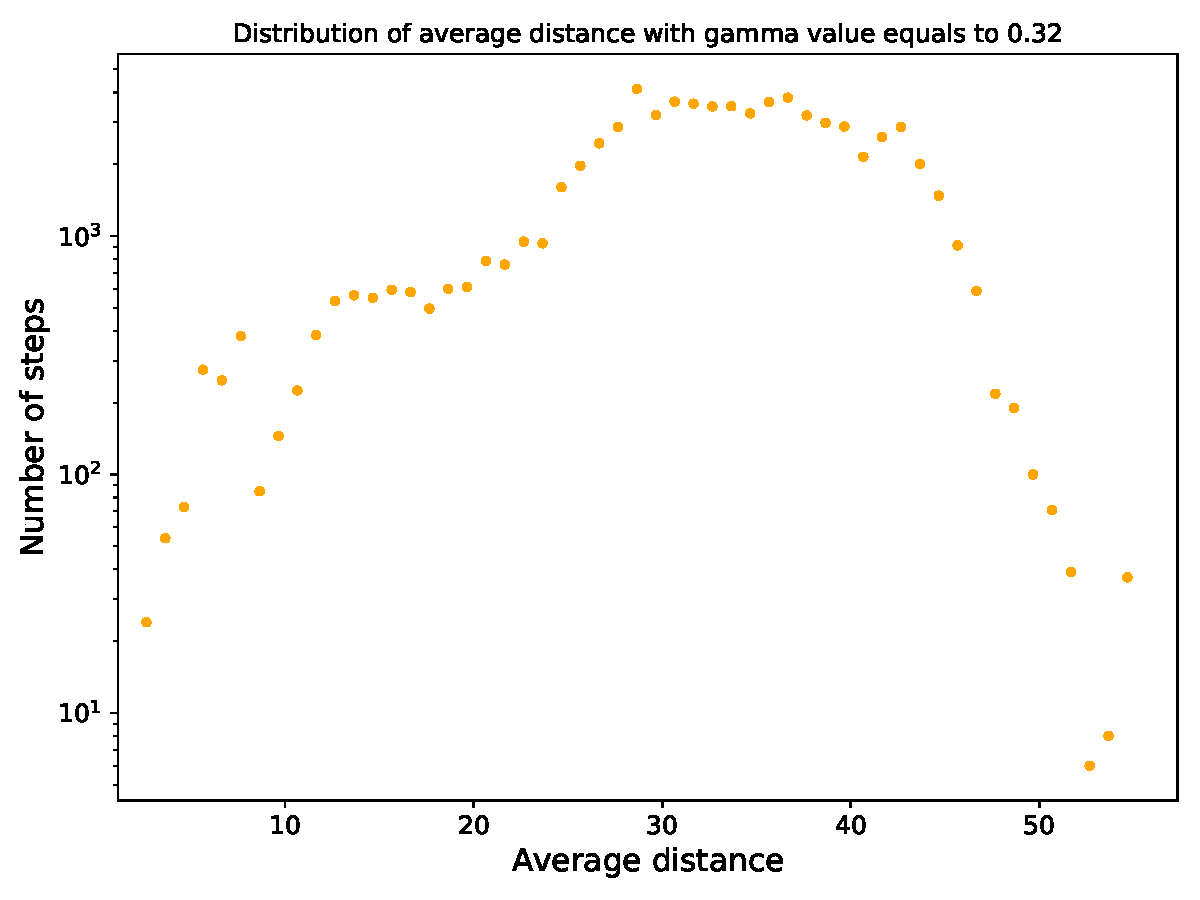
\includegraphics[width=.47\linewidth]{images/gamma_results/high_alpha/distribution_distance_gamma_0_32}
	}
	\hfill
	\subfloat[Distribuzione della distanza media mantenuta dai robot con un valore di $\gamma$ pari a 0.65.\label{sfig:gammaHDistr0.65}]{
		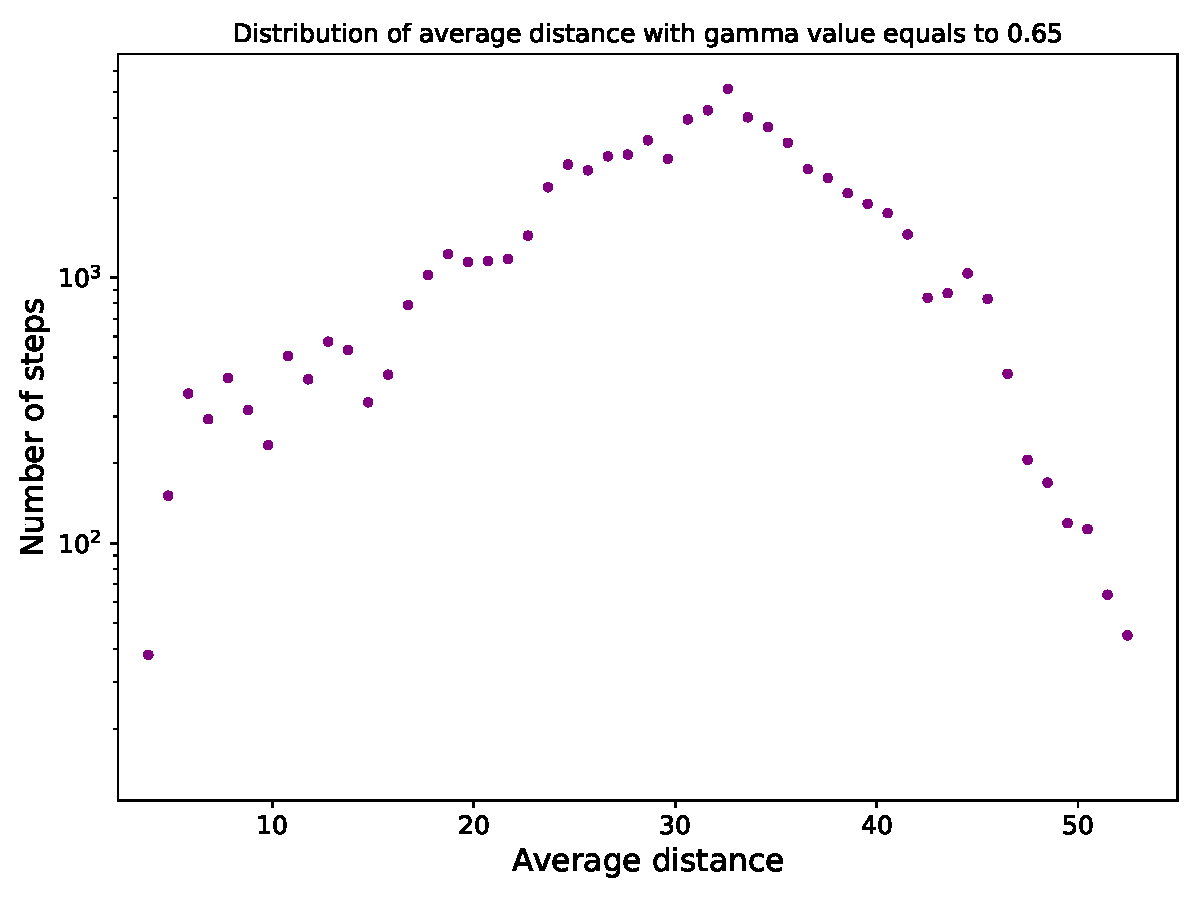
\includegraphics[width=.47\linewidth]{images/gamma_results/high_alpha/distribution_distance_gamma_0_65}
	}
	\caption{Distribuzione della distanza media mantenuta dai robot al variare del valore di $\gamma$, per valutare la distribuzione si è conteggiato in quanti \textit{step} i robot hanno presentato tale distanza, il numero di \textit{bin} per produrre la distribuzione è pari alla differenza tra la distanza minima e massima presente durante la simulazione, tale valore è stato poi arrotondato. Infine si noti che l'asse delle \textit{y} è a scala logaritmica.}
	\label{fig:gammaHDistr}
\end{figure}
Ancora una volta si è deciso di andare a confrontare tutte le distribuzioni dei valori del parametro analizzati, i risultati sono mostrati in Figura \ref{fig:gammaHComparison}.
Come si può notare, al contrario del caso precedente, per valori pari a 0.65 o 1 si notano dei “picchi” significativi e anche per valori più bassi (0.1 e 0.32) si nota come i robot mantengano una distanza media maggiore; tale risultato sembra contraddire quello detto in precedenza.\\
Per analizzare meglio questi risultati e introdurli nel quadro complessivo, bisogna considerare che non è solo $\gamma$ (come avveniva di fatto precedentemente) ad influire sulla scelta della cella obiettivo e degli spostamenti del robot, ma risulta essere vincolante anche il costo del cammino. 
Poiché il parametro $\alpha$ influisce significativamente e con una magnitudo molto maggiore rispetto all'utilità e priorità della cella nella scelta del bersaglio, il parametro $\gamma$ passa in secondo piano e influisce solo in maniera marginale sulla scelta. Ciò va ad inficiare la distanza tra i robot, poiché tali scelte non vengono più effettuate dando grande importanza all'utilità della cella quanto al tempo necessario per raggiungerla.
\begin{figure}
	\centering
	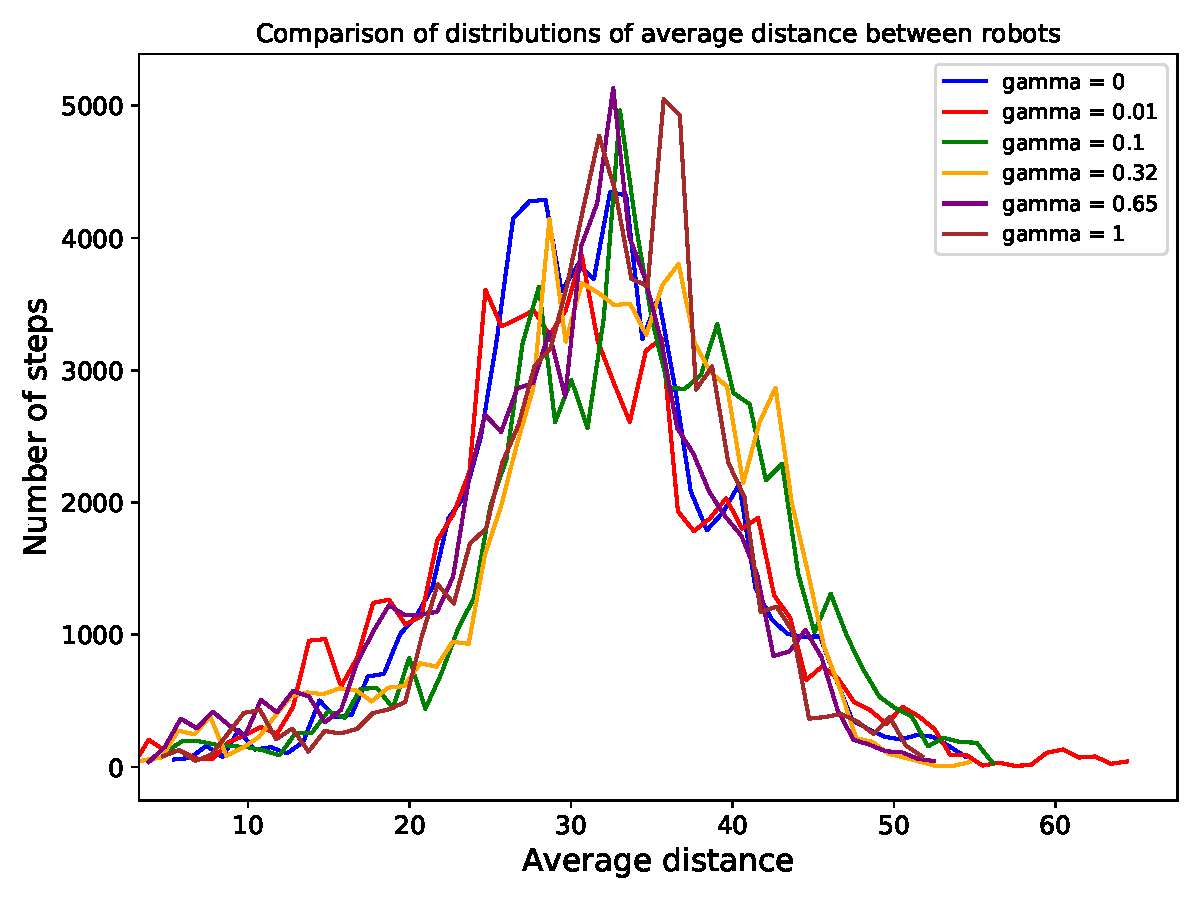
\includegraphics[width=0.9\linewidth]{images/gamma_results/high_alpha/comparison}
	\caption{Grafico che riassume tutte le distribuzioni di distanze medie durante le simulazioni per ogni valore di $\gamma$, si noti che l'asse delle \textit{y} non è più logaritmico.}
	\label{fig:gammaHComparison}
\end{figure}
Come ulteriore conferma di tale affermazione, si può notare come durante la singola simulazione non si presentino più quelle situazioni in cui la distanza tra i robot decresce significativamente a causa della segnalazione da parte dei feriti. Solo durante le fasi finali dell'esplorazione la distanza tra essi alle volte diminuisce.
Al fine di evitare che i feriti vengano di fatto ignorati, è stata implementata una seconda tecnica di prioritizzazione delle celle che, al posto di utilizzare un valore fisso stabilito a priori, utilizza un valore dipendente da $\alpha$; i risultati di tale metodo, discusso nella Sotto-sezione \ref{Ferito} saranno discussi tra breve.
L'evolversi delle distanze è rappresentato in Figura \ref{fig:gammaHSim}
\begin{figure}
	\subfloat[Evoluzione della distanza media tra gli agenti con un valore di $\gamma$ pari a 0.32.]{
		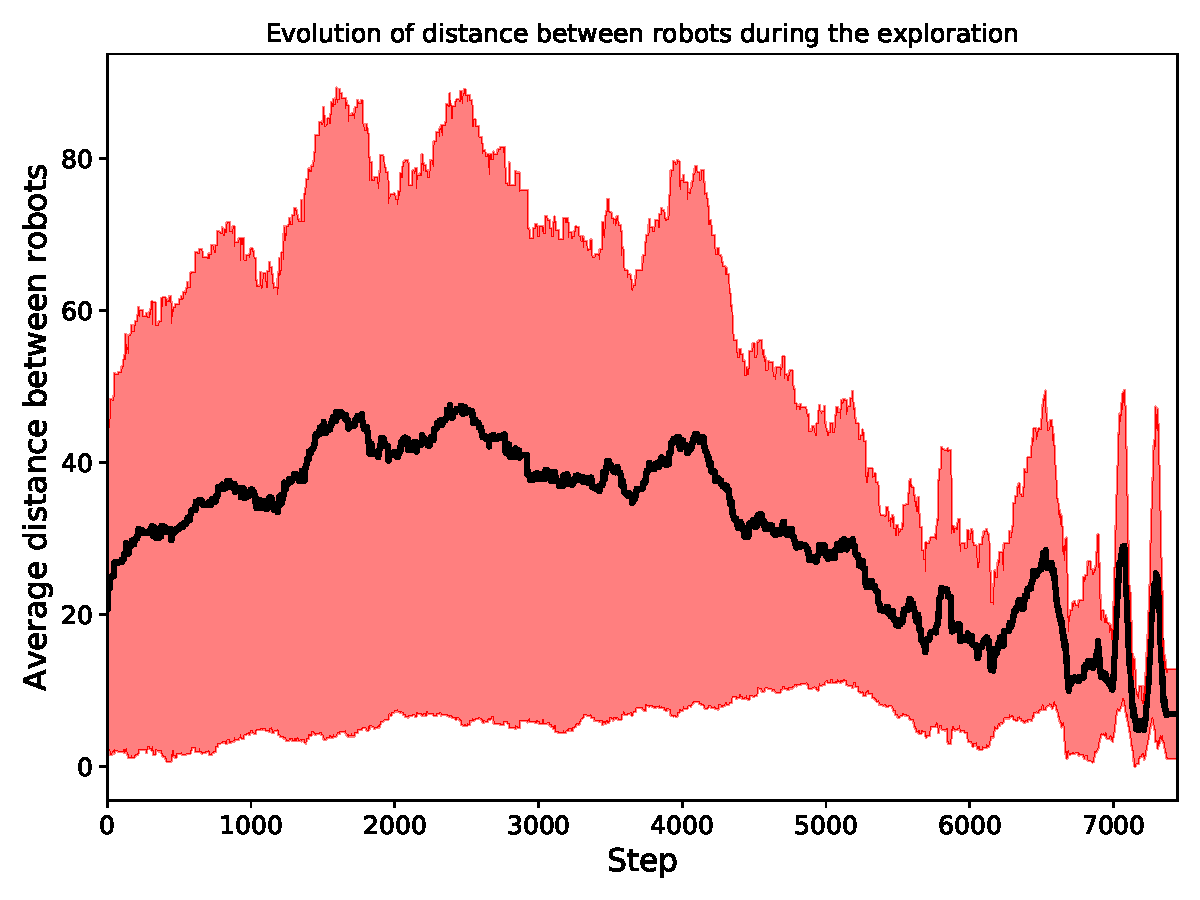
\includegraphics[width=.47\linewidth]{images/gamma_results/high_alpha/dinstance_simulation_gamma_0_32_simid_0}
	}
	\hfill
	\subfloat[Evoluzione della distanza media tra gli agenti con un valore di $\gamma$ pari a 0.65.]{
		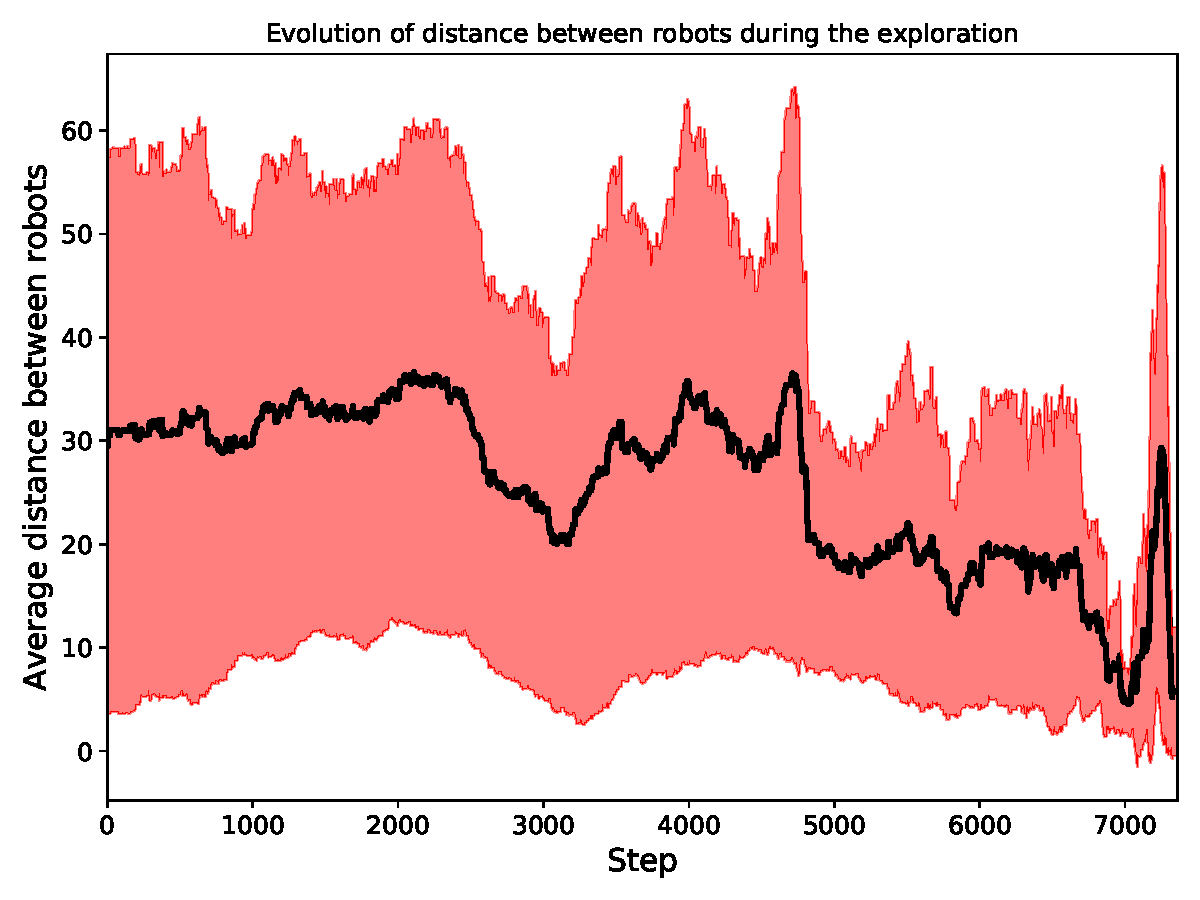
\includegraphics[width=.47\linewidth]{images/gamma_results/high_alpha/dinstance_simulation_gamma_0_65_simid_4}
	}
	\caption{Sull'asse delle \textit{x} si trova il tempo, in termini di \textit{step}, impiegato per l'esplorazione della mappa, mentre sull'asse delle \textit{y} la distanza media tra gli agenti.}
	\label{fig:gammaHSim}
\end{figure}
\subsection{Considerazioni conclusive}
In questo breve sunto, si vogliono evidenziare alcune differenze tra come opera il parametro $\gamma$ rispetto al valore di $\alpha$.
In particolare, si è notato come per valori di $\alpha$ bassi è effettivamente il parametro $\gamma$ ad influire sulla distanza tra i robot portando questi a scegliere le celle con utilità maggiore (poiché il peso influisce in maniera poco significativa) e quindi scegliendo le celle viste da meno robot (poiché sono quelle che hanno subito meno riduzioni di utilità).
In aggiunta, si evidenzia come per valori di $\alpha$ bassi i robot tenderanno a muoversi tutti verso la zona segnalata da un ferito nel momento in cui questi segnalano la loro presenza; al contempo, tale effetto sembra più marginale nel momento in cui $\alpha$ aumenta.
Nonostante queste considerazioni, si nota comunque come per valori di $\gamma$ elevati gli agenti, in entrambi i casi, tendono a rimanere più distanti rispetto a valori bassi (si tenga presente che i “picchi” per $\alpha$ elevati sono presenti per valori di distanza minori).
Ancora una volta, tale fenomeno è dovuto al fatto che quando il costo del cammino è maggiormente significativo nel calcolo dell'\textit{info-gain} diventa il principale parametro che delinea la scelta e quindi riducendo l'effetto dell'utilità delle celle e di conseguenza l'influenza del parametro $\gamma$.
\subsection{Metodo di prioritizzazione alternativo}
Al fine di indagare come il metodo di prioritizzazione alternativo, proposto nella Sotto-sezione \ref{subsec:Ferito}, fosse in grado di modificare il comportamento dei robot negli scenari analizzati in precedenza, sono stati ripetuti i medesimi test utilizzando però la forma di priorità che tiene conto del valore di $\alpha$. Questo dovrebbe portare i robot a evitare situazioni in cui l'intera flotta si raduna in un unico punto a seguito della segnalazione della presenza di un ferito (comportamento evidenziato con valori di $\alpha$ bassi).
Come mostrato nella Figura \ref{fig:NgammaLDistr}, i dati sembrano confermare quanto supposto. Non sono più evidenti decrescite repentine che portano i robot a raggrupparsi in una medesima area, come era invece mostrato nell'analisi corrispettiva eseguita con il precedente metodo di prioritizzazione (Figura \ref{fig:gammaSim})
\begin{figure}
	\subfloat[Evoluzione della distanza media tra gli agenti con un valore di $\gamma$ pari a 0.32.]{
		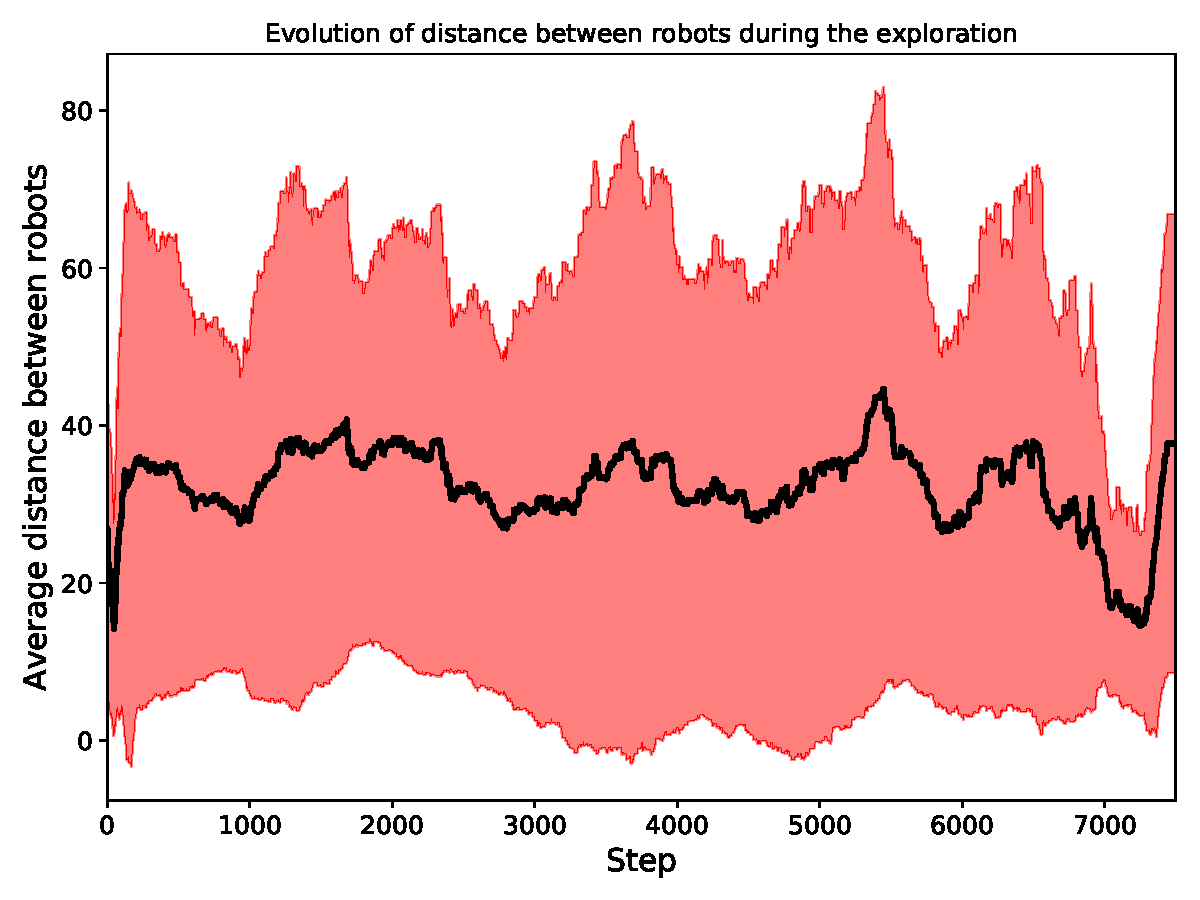
\includegraphics[width=.47\linewidth]{images/high_priority_gamma_results/low_alpha/dinstance_simulation_gamma_0_32}
	}
	\hfill
	\subfloat[Evoluzione della distanza media tra gli agenti con un valore di $\gamma$ pari a 0.65.]{
		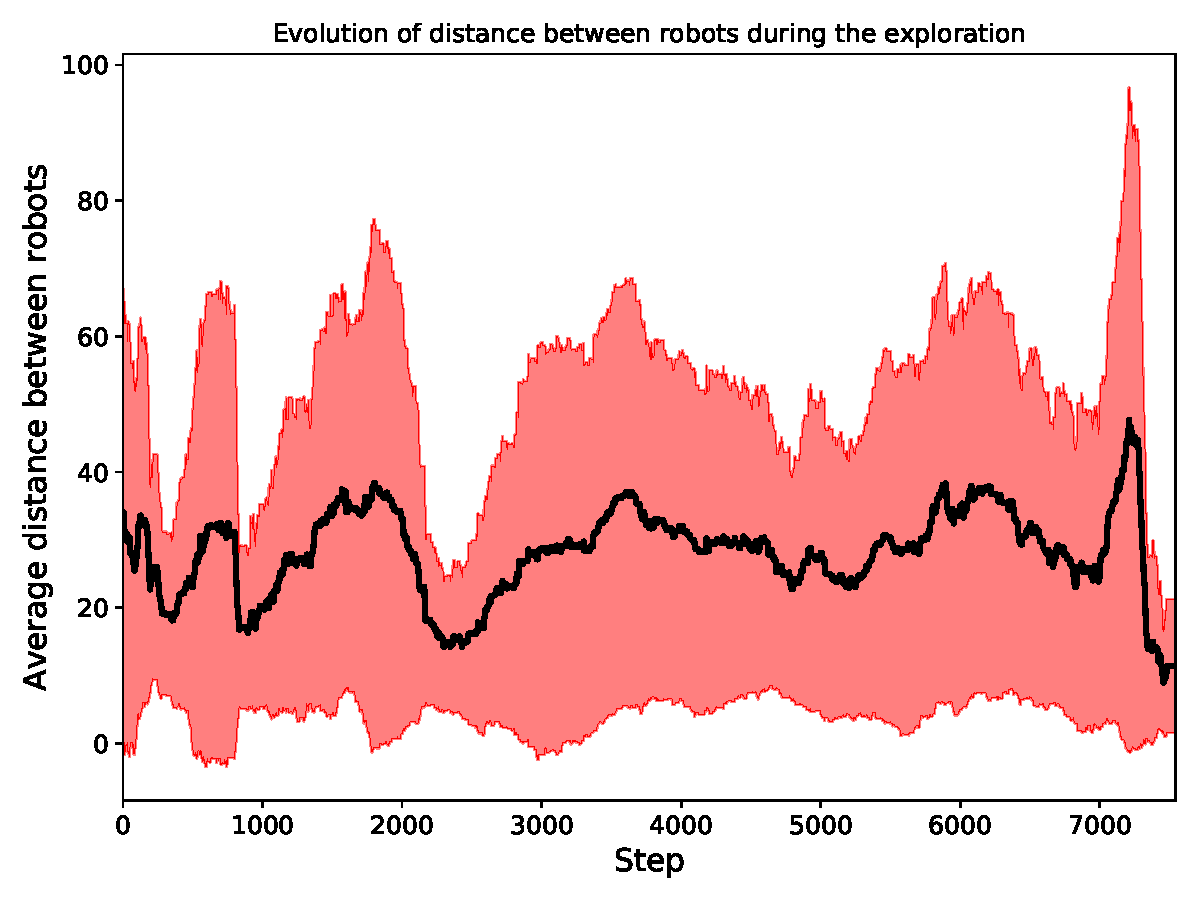
\includegraphics[width=.47\linewidth]{images/high_priority_gamma_results/low_alpha/dinstance_simulation_gamma_0_65}
	}
	\caption{Sull'asse delle \textit{x} si trova il tempo, in termini di \textit{step}, impiegato per l'esplorazione della mappa, mentre sull'asse delle \textit{y} la distanza media tra gli agenti.}
	\label{fig:NgammaLDistr}
\end{figure}
Al contempo, analizzando il grafico comparativo delle distribuzioni di distanza tra i robot ad ogni \textit{step}, riportato in Figura \ref{fig:NgammaLComparison}, vediamo come vi sia un'effettiva minore distanza media per valori di $\gamma$ prossimi a zero rispetto agli altri casi. Questo avvalora la tesi già enunciata in precedenza che sostiene che valori di gamma prossimi al valore nullo portano tutte le celle nel vicinato della cella obiettivo, anche quelle molto distanti, ad avere utilità simile e prossima a zero. Ciò porta il costo del cammino minimo verso l'obiettivo a diventare nuovamente protagonista nel calcolo dell'\textit{info-gain}, rendendo vana la tecnica di repulsione tra robot così implementata.
\begin{figure}
	\centering
	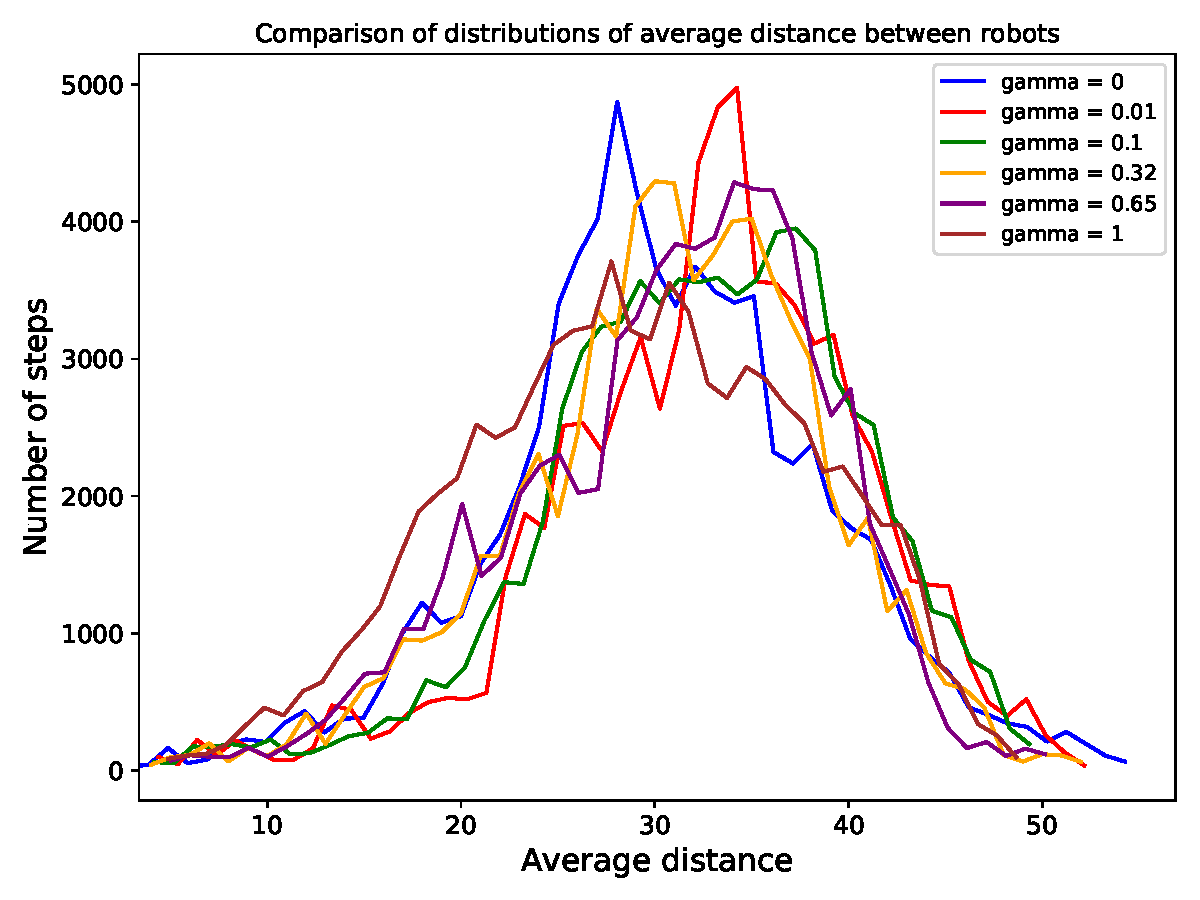
\includegraphics[width=0.9\linewidth]{images/high_priority_gamma_results/low_alpha/comparison}
	\caption{Grafico che riassume tutte le distribuzioni di distanze medie durante le simulazioni per ogni valore di $\gamma$, si noti che l'asse delle \textit{y} non è più logaritmico.}
	\label{fig:NgammaLComparison}
\end{figure}
Per quanto concerne i dati ottenuti con valori di $\alpha$ più elevati, i risultati e le conclusioni sono assimilabili a quelle appena tratte per valori del parametro inferiori (tutti i grafici sono disponibili nell'Appendice \ref{apx:gamma}).

\newpage
\section{Stato dei robot}
\label{sec:status}
Un'ultima analisi effettuata è stata riguardo lo stato degli agenti durante il processo di esplorazione della mappa.
In particolare, si è studiato per ogni \textit{step} di una simulazione il numero di agenti che fossero nei seguenti stati:
\begin{itemize}
	\item esplorazione di una cella;
	\item movimento verso una cella;
	\item rilascio un ripetitore;
	\item scelta della prossima cella obiettivo o attesa dell'aggiunta di celle obiettivo.
\end{itemize}
Per raccogliere tali dati, è stata effettuata una singola simulazione su due mappe particolari generate \textit{ad hoc} e 5 mappe casual che non presentassero casi patologici.
Tutte le mappe sono di dimensione 30$\times$30, per questioni di tempo richiesto dalle singole simulazioni, $\alpha$ e $\gamma$ assumono valori pari ai valori indotti dal processo di ottimizzazione (Sezione \ref{sec:psoResults}), il raggio di percezione pari a 6 celle e quello dei ripetitori pari a 3 celle.
Inoltre, sono stati utilizzati 6 robot e i feriti potevano segnalare la loro presenza.\\
Le prima delle due mappe particolari rappresenta una situazione che vuole simulare la presenza di un ponte, ovvero si può considerare la mappa divisa in due parti che sono unite solo da una piccola porzione di terra attraversabile.
La seconda è una mappa che presenta delle zone non raggiungibili, non visibili e, quindi, non esplorabili.

I risultati raccolti sono riportati in Figura \ref{fig:status}; si noti che per rendere i dati leggibili sono stati calcolati 100 intervalli in cui suddividere i dati e questi ultimi sono stati aggregati all'interno di ogni intervallo. Per questo motivo in colore si notano le medie e in nero le relative \textit{errorbar}.
Dai grafici, si può dedurre come la maggior parte dei robot siano quasi sempre impegnati nell'esplorazione e passano poco tempo nelle altre fasi. Questo indica che i robot tendono sempre a scegliere le celle più economiche da raggiungere (poiché il valore del parametro $\alpha$ è elevato) e che passano la maggior parte del tempo a esplorare le celle.
Se così non fosse, ci sarebbe un numero medio di robot minore in fase di esplorazione.
Si può, infine, notare come la fase di rilascio dei ripetitori sia un'attività in cui tipicamente solo uno dei robot è impegnato, indicando quindi che la costruzione della rete \textit{mesh} non sia un collo di bottiglia che aumenta significativamente i tempi di esplorazione del territorio.
Infine, si faccia riferimento all'Appendice \ref{apx:status} per i grafici non qui rappresentati.

\begin{figure}
	\begin{tabular}{cc}
		\subfloat[Stato dei robot durante l'esplorazione della mappa con il ponte.]{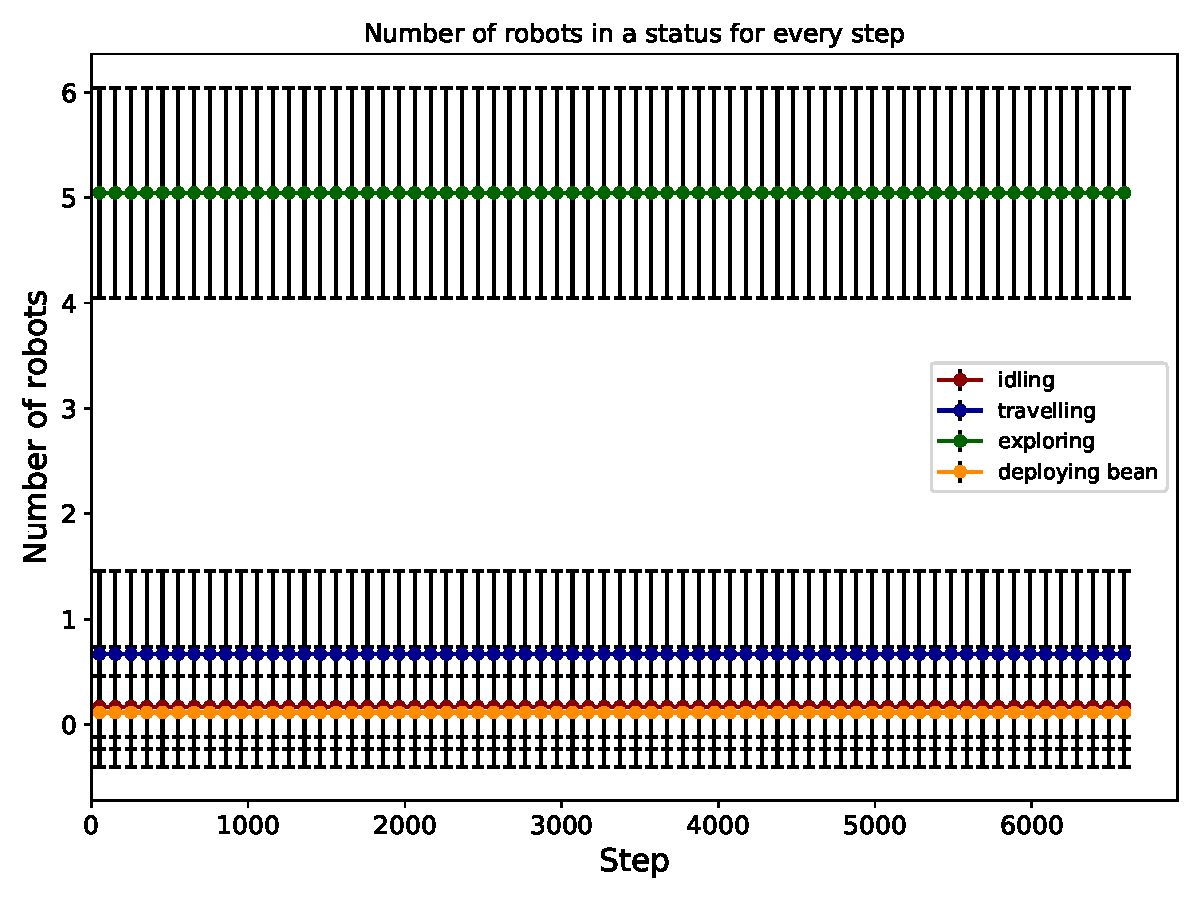
\includegraphics[width = .5\textwidth]{images/status_results/bridge_sim0}} &
		\subfloat[Stato dei robot durante l'esplorazione della mappa con zone non raggiungibili.]{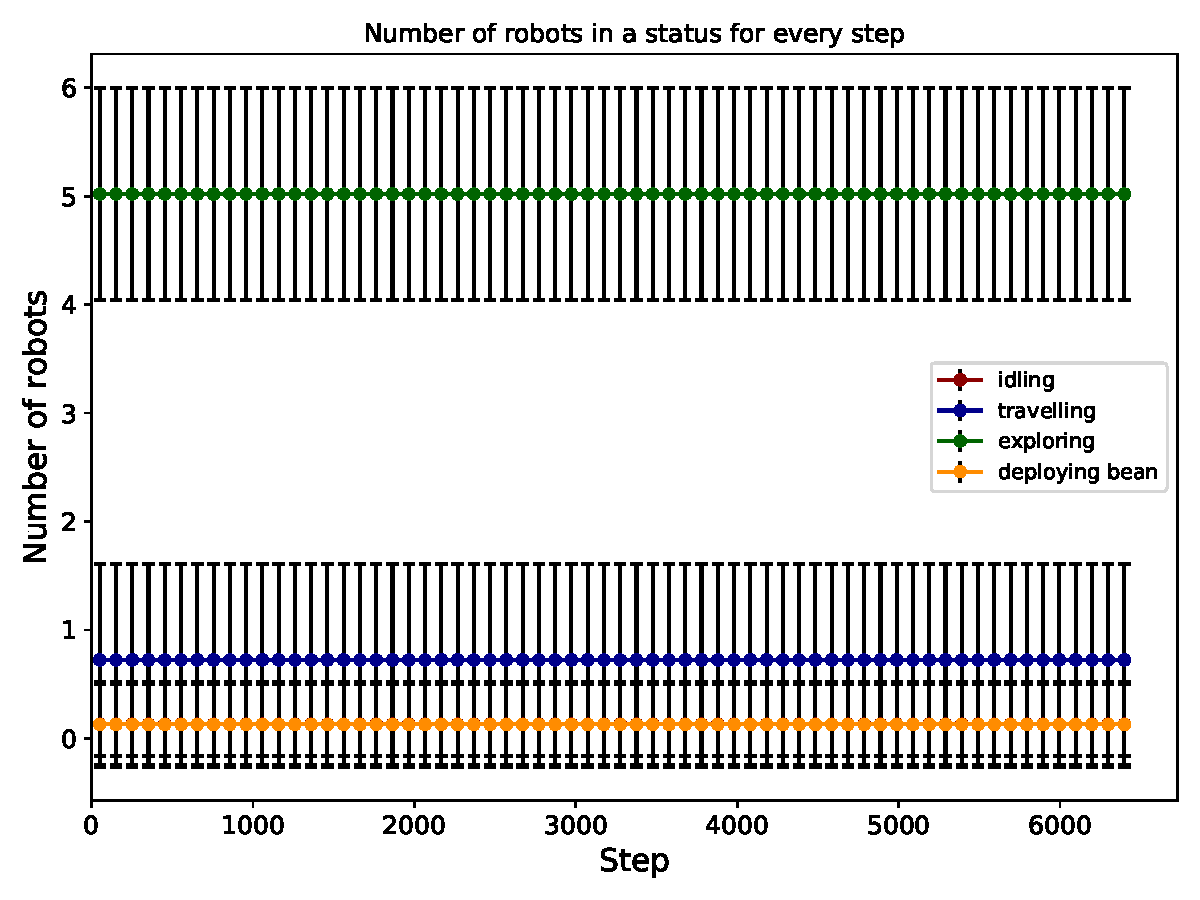
\includegraphics[width = .5\textwidth]{images/status_results/buildings_sim0}}\\
		\subfloat[Stato dei robot durante l'esplorazione della mappa generata casualmente numero 2.]{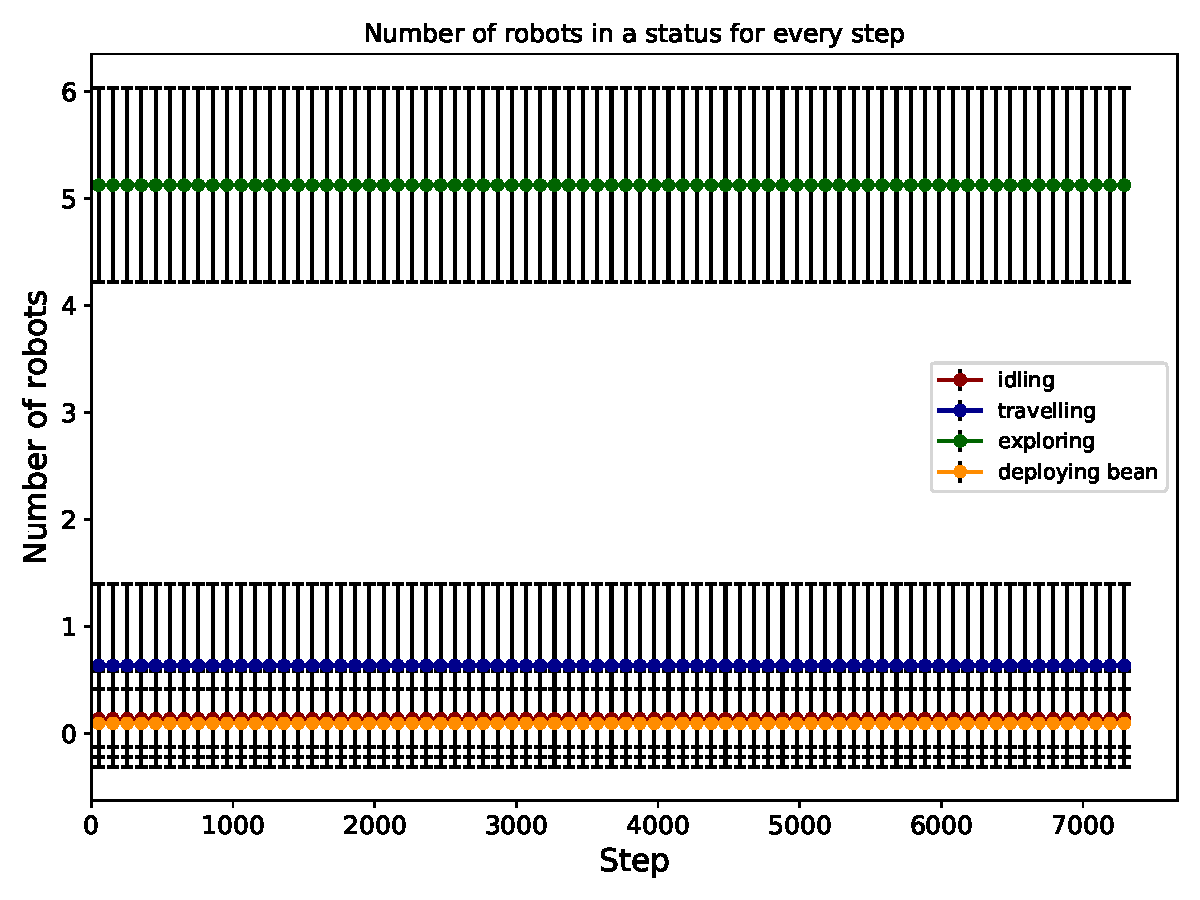
\includegraphics[width = .5\textwidth]{images/status_results/random2_sim0}} &
		\subfloat[Stato dei robot durante l'esplorazione della mappa generata casualmente numero 5.]{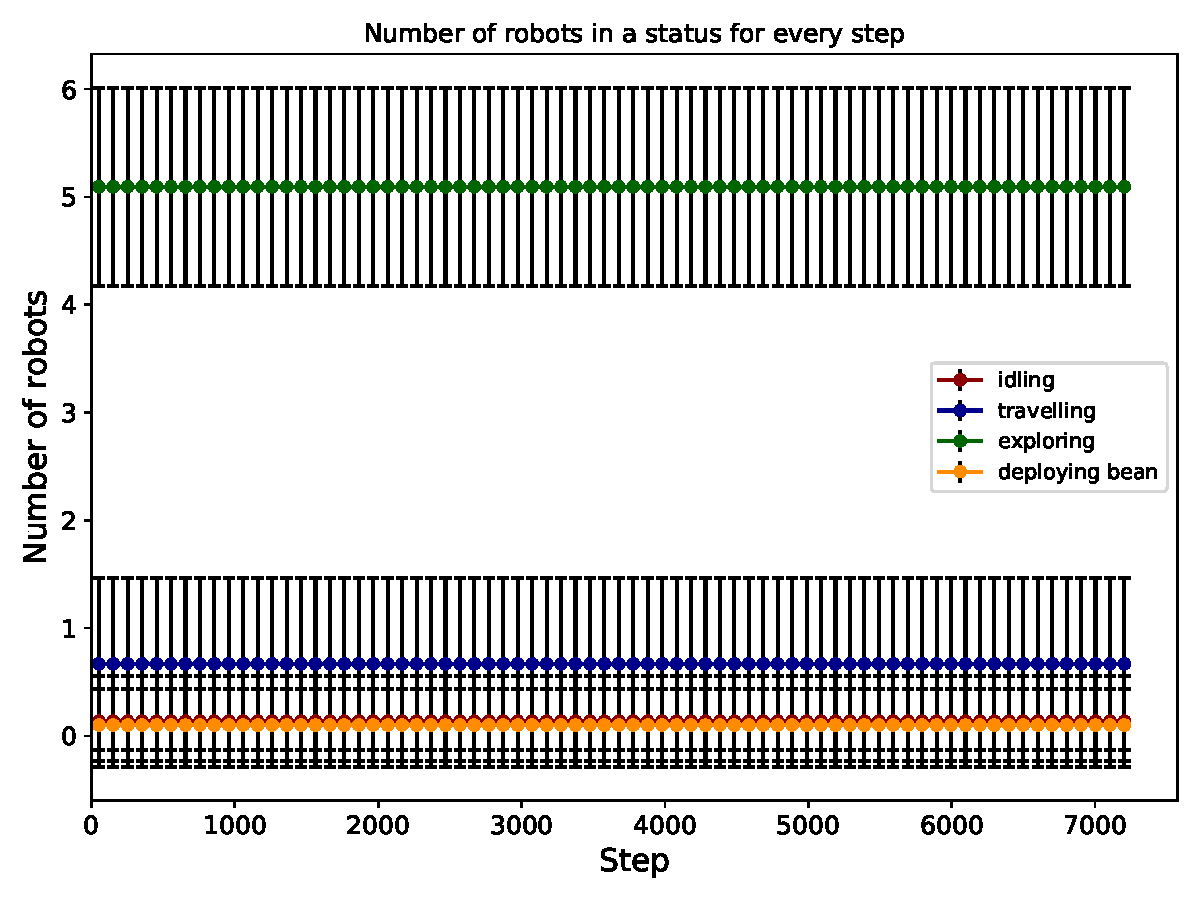
\includegraphics[width = .5\textwidth]{images/status_results/random5_sim0}}\\
	\end{tabular}
	\caption{Sull'asse delle \textit{x} si trova il tempo, in termini di \textit{step}, impiegato per l'esplorazione della mappa, mentre sull'asse delle \textit{y} il numero di agenti in un determinato stato. Si noti che i dati sono stati raggruppati per formare 100 \textit{bin} in modo da rendere leggibile il grafico; di conseguenza, in colore si trovano le medie e le \textit{errorbar} rappresentano le devizioni standard rispeto alla media.}
	\label{fig:status}
\end{figure}